
\documentclass[titlepage,11pt,a4paper]{report}
%\usepackage[titlepage, fancysections]{polytechnique}
\usepackage[utf8]{inputenc} 
\usepackage[T1]{fontenc}
\usepackage[english]{babel}
\usepackage[toc,page]{appendix}
\usepackage{graphicx}
\usepackage[colorinlistoftodos]{todonotes}


\usepackage{todonotes}
\usepackage{hyperref}
\usepackage{url}
\usepackage{caption}
\usepackage{subcaption}
\usepackage{float}
\usepackage{amsmath, amssymb, stmaryrd, bussproofs, amsthm}
\usepackage{tikz}
\usepackage{booktabs} 
\usepackage{subcaption}
\usepackage[nottoc]{tocbibind}
\usepackage{dashbox}
\usepackage{listings}
\usepackage{mathtools}
\usepackage{xcolor}
\lstset { %
	tabsize=2,
    language=C++,
    backgroundcolor=\color{black!5}, % set backgroundcolor
    basicstyle=\footnotesize,% basic font setting
}
\usepackage{tikz}
\usetikzlibrary{matrix, fit, calc}

\title{Verifying weak memory programs in the Viper ecosystem} 

\author{Anouk Paradis}

%\date{July, 2018}



\theoremstyle{plain}
\newtheorem{theorem}{Theorem}[section]
\newtheorem{definition}{Definition}
\newtheorem{lemma}[theorem]{Lemma}
\newtheorem{proposition}[theorem]{Proposition}
\newtheorem{corollary}{Corollary}
\usepackage{afterpage}

\newcommand\ghost[1]{\dbox{\ensuremath{#1}}}
\newcommand\rPerm{R_{\lambda}^{EFC}(\text{bits})}
\newcommand\wPerm{W_{\lambda}^{EFC}(\text{bits})}
\newcommand\Uperm{\{\text{U}(\text { bits }, \mathcal{Q})\}}
\newcommand\emp{\mathrm{emp}}
\newcommand\ress[1]{resource(\texttt{bits})^{#1}} 
\newcommand\efcp[2]{\ghost{\lambda :(#1, #2)^{+}}}
\newcommand\efcm[2]{\ghost{\lambda :(#1, #2)^{-}}}
\newcommand\acqPerm{\operatorname{\mathsf{Acq}}(\ell, \mathcal{Q})}
\newcommand\acqPermp[1]{\operatorname{\mathsf{Acq}}(\ell, \mathcal{Q}_{#1})}
\newcommand\relPerm{\operatorname{\mathsf{Rel}}(\ell, \mathcal{Q})}
\newcommand\rmwPerm{\operatorname{\mathsf{RMWAcq}}(\ell, \mathcal{Q})}


\newcommand\consQ{\mathsf{Consumer}(\texttt{s.queue})}
\newcommand\prodQ{\mathsf{Producer}(\texttt{s.queue})}
\newcommand\sePred{\mathsf{SE}_\gamma(s)}


\newcommand\blankpage{%
    \null
    \thispagestyle{empty}%
    \addtocounter{page}{-1}%
    \newpage}

\begin{document}

\begin{titlepage}

\newcommand{\HRule}{\rule{\linewidth}{0.5mm}} % Defines a new command for the horizontal lines, change thickness here

\center % Center everything on the page
 
%----------------------------------------------------------------------------------------
%   HEADING SECTIONS
%----------------------------------------------------------------------------------------

%\textsc{\LARGE \'Ecole polytechnique}\\[1.5cm] % Name of your university/college
\textsc{\Large Research in Computer Science Project Report}\\[0.5cm] % Major heading such as course name
%\textsc{\Large Non confidential}\\[0.5cm] % Major heading such as course name
%\textsc{\large Minor Heading}\\[0.5cm] % Minor heading such as course title

%----------------------------------------------------------------------------------------
%   TITLE SECTION
%----------------------------------------------------------------------------------------

\HRule \\[0.4cm]
{ \huge \bfseries Verifying weak memory programs in the Viper ecosystem}\\[0.4cm] % Title of your document
\HRule \\[1.5cm]


 
%----------------------------------------------------------------------------------------
%   AUTHOR SECTION
%----------------------------------------------------------------------------------------

\begin{minipage}{0.4\textwidth}
\begin{flushleft} \large
\emph{Author:}\\
Anouk \textsc{Paradis} \\% Your name 
\small
Master of Computer Science\\
ETH
\end{flushleft}
\end{minipage}
~
\begin{minipage}{0.4\textwidth}
\begin{flushright} \large
\emph{Supervisors:} \\
Gaurav \textsc{Parthasarathy}\\ % Supervisor's Name
\small
PM Group\\
ETH\\
\textcolor{white}{lala}\\

\large
Pr.~Alexander J.\textsc{Summers}\\ % Supervisor's Name
\small
PM Group\\
ETH
\end{flushright}
\end{minipage}\\[2cm]

% If you don't want a supervisor, uncomment the two lines below and remove the section above
%\Large \emph{Author:}\\
%John \textsc{Smith}\\[3cm] % Your name

%----------------------------------------------------------------------------------------
%   DATE SECTION
%----------------------------------------------------------------------------------------

{\large \today}\\[2cm] % Date, change the \today to a set date if you want to be precise

%----------------------------------------------------------------------------------------
%   LOGO SECTION
%----------------------------------------------------------------------------------------

%\includegraphics[width=3cm]{/home/anouk/2018/packageLatexPolytechnique/source/polytechnique-logovert.pdf}\\[1cm] % Include a department/university logo - this will require the graphicx package
 
%----------------------------------------------------------------------------------------

\vfill % Fill the rest of the page with whitespace

\afterpage{\blankpage}

\end{titlepage}


%\begin{abstract}
%		idkls;adkls;a
%\end{abstract}


\tableofcontents

\afterpage{\blankpage}

%Bien relus: intro, ch1 et ch2
%A relire background et ccl
%A reprendre d'apres rqs de Gaurav: ch3

\chapter{Introduction}
When reasoning about concurrent programs, the most intuitive setting is sequential consistency \cite{LamportSC}, where we consider the program to behave as if each of the threads' executions were simply interleaved. However, due to the many optimizations performed by modern compilers and hardware, such a model is too simplistic to accurately represent the actual executions of the program. We can hence only assume a weak memory model, which allows many more possible executions of the accesses to shared memory locations. However, these new possibilities of execution make reasoning about programs more difficult, and at times counterintuitive. Writing correct programs is hence extremely challenging in such a setting.

FSL++ \cite{fsl} is a program logic developed to reason about concurrent programs in C11, which are governed by the weak memory model defined in the C11 standard. This program logic allows for compositional proofs, through preconditions and postconditions for functions for instance. However, such proofs originally had to be encoded using the Coq interactive theorem prover, thus requiring a lot of ad hoc work for each new program considered.

%While these logics have successfully been used to prove some programs taken from real-world libraries, for instance in \cite{rcu}, these proofs still require a lot of ad-hoc work for each new program considered, as each proof has to be encoded in the Coq interactive theorem prover.

To try to alleviate this proof burden, part of this program logic has been encoded into Viper \cite{viper} by Summers and M\"uller \cite{rslViper}. However it did not provide any encoding for the notion of custom \emph{ghost state}, an important feature used to model information that cannot be deduced solely from the program state. This \emph{ghost state} is defined quite generally in FSL++, and needs to be specialized for each example, which makes their encoding and their use quite challenging. Parthasarathy et al. \cite{gaurav} provided such a specialization, the EFC permission structure, and showed that it was sufficient to prove the correctness of a variety of example programs. Building on this work, Wiesmann et al. \cite{pascal} was then able to define a specification syntax, token based reasoning, and its encoding in Viper. This syntax abstracts some details of the EFC ghost state and FSL++, such as rational permission amounts, limiting the complexity of this logic.
%, that allowed easier use of this specialization, without having to deal with lower level details. 
Wiesmann et al. \cite{pascal} also implemented a C++ front end for Viper using this specialization to provide more automation for proofs.  

This project explores this new infrastructure and tries to analyze some of its limitations, not only in terms of what it allows us to do, but also in how easily it allows us to do it. We were first able to identify a slight mismatch between the intuition of the EFC permission structure and token based reasoning. Furthermore, we found and studied three new real-world examples. The first two allowed us to identify strong limitations of FSL++ that forbid proving many kind of examples. We finally provide a proof of the last example, that uses two atomic locations, using the EFC permission structure. 

\chapter{Background}
\label{ch:background}
%In this section we give the background needed to better understand the upcoming part of this report. 

\section {Weak Memory}
As explained in the introduction, we cannot expect a sequentially consistent behavior from any parallel program. 
%However, dealing with the behaviors introduced by weak memory is cumbersome and error-prone. Libraries hence contain all the necessary locks and synchronization tools, that if used properly ensure a sequentially consistent behavior. Hence only those writing those libraries have to deal with weak memory.
We have to deal with all the behaviors introduced by weak memory. We will now explain in some more details how those work.

We consider two types of memory locations: atomics and non atomics. Non atomics are the default, the ones we use in most programs. However, they are not adapted for concurrent access: if two threads try to access a non atomic location at the same time, and at least one of them intends to write, there is a data race, and the behavior of the program is undefined. Hence we cannot use this kind of locations in a concurrent environment without making sure that no such racy access can happen. 

The required synchronization is done using atomics. Operations on those locations are atomic: we can think of them as happening in an instant, so that nothing can happen at the same time (since they took so little time). Hence the race situation described above, with a thread reading from an atomic location at the same time as another thread is writing to it, cannot happen. As both operations are atomic, either the read happens first, or the write does. However, those atomic operations are more expensive than non atomic ones. Hence we only use them to create the necessary synchronization to avoid data races.

\subsection{Synchronization on atomics}
While atomics are unaffected by races, we still cannot trust them for sequential consistency. Due to potential reorderings by the compiler or the processor, or delayed synchronization of different caches, \texttt{a = 1; b = 1} may become \texttt{b = 1; a = 1}. We hence need some construct to enforce ordering between memory accesses, be them atomic or non atomic. We use fences for that. We here only mention three of them: sequentially consistent (SC) ones, acquire (Acq) ones and release (Rel) ones. The synchronization they offer is summarized in Figure~\ref{fig:fence}. The sequentially consistent fence is the stronger of them all: it forbids any reodering around it. However, it is quite expensive. Hence, most of the time we try to use weaker fences, that take less time to enforce. The release fence ensures that any read or write before it will not be re-ordered after the writes after it. Hence reading a value written by a write after this fence guarantees that all memory operations that happened before this fence are visible as well: they were \emph{released} with the write. The acquire fence ensures that any read before it will not be re-ordered with any read or write after it.

\begin{figure}
\begin{tabular}{ccc}
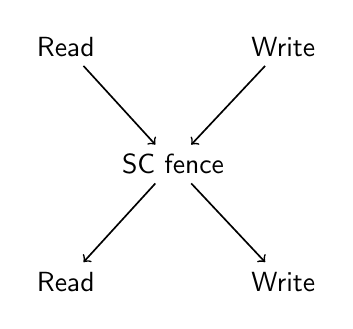
\begin{tikzpicture}[font=\sffamily]
    \node (f) at (0,0) {SC fence};
    \node (rA) [above left=1cm and 0.1cm of f]  {Read};% 2cm below, 1cm to the left (optional)
    \node (wA) [above right=1cm and 0.1cm of f] {Write};
    \node (rB) [below left=1cm and 0.1cm of f]  {Read};
	\node (wB) [below right=1cm and 0.1cm of f] {Write};
    \draw [semithick,->] (rA) -- (f);
    \draw [semithick,->] (wA) -- (f);
    \draw [semithick,->] (f) -- (rB);
    \draw [semithick,->] (f) -- (wB);
\end{tikzpicture}
		& 
		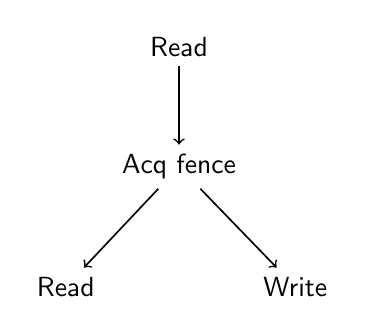
\begin{tikzpicture}[font=\sffamily]
    \node (f) at (0,0) {Acq fence};
    \node (rA) [above= 1cm of f]  {Read};% 2cm below, 1cm to the left (optional)
    %\node (wA) [above right=1cm and 1cm of f] {Write};
    \node (rB) [below left=1cm and 0.1cm of f]  {Read};
	\node (wB) [below right=1cm and 0.1cm of f] {Write};
    \draw [semithick,->] (rA) -- (f);
    %\draw [semithick,->] (wA) -- (f);
    \draw [semithick,->] (f) -- (rB);
    \draw [semithick,->] (f) -- (wB);
\end{tikzpicture}
	
		&
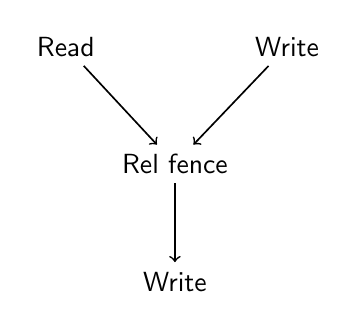
\begin{tikzpicture}[font=\sffamily]
    \node (f) at (0,0) {Rel fence};
    \node (rA) [above left=1cm and 0.1cm of f]  {Read};% 2cm below, 1cm to the left (optional)
    \node (wA) [above right=1cm and 0.1cm of f] {Write};
    %\node (rB) [below left=1cm and 1cm of f]  {Read};
	\node (wB) [below=1cm of f] {Write};
    \draw [semithick,->] (rA) -- (f);
    \draw [semithick,->] (wA) -- (f);
    %\draw [semithick,->] (f) -- (rB);
    \draw [semithick,->] (f) -- (wB);
\end{tikzpicture}
	
\end{tabular}
\caption{Fences synchronization}
\label{fig:fence}
\end{figure}

The easiest way to think about how those fences work, is to consider that the order in which different operations appear in the program have no impact on their actual execution order unless we use some special construct that enforces an order. This is kind of the way the \emph{happen-before} relation defined in the C11 standard works \cite{C11}: we assume no order, and define using fences, operations reading on the same variable, ... a transitive relation that explicits the order that is preserved during the actual execution. Using this way of thinking, a release fence creates arrows from all read and writes above it to itself, and from itself to all writes below it.

On top of the fences, we can enforce synchronization by doing a \emph{release write} or an \emph{acquire read}. Here the synchronization is slightly weaker than when using a fence, as shown on Figure~\ref{fig:readWrite}. For instance, the release write only forbids reordering of previous read or writes with itself, and not with all writes after itself. 
\begin{figure}
\begin{tabular}{cc}
		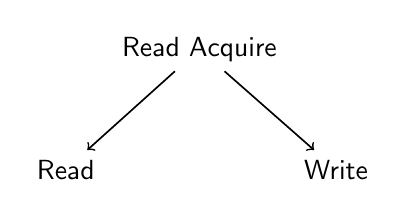
\begin{tikzpicture}[font=\sffamily]
    \node (f) at (0,0) {Read Acquire};
    %\node (rA) [above= 1cm of f]  {Read Acquire};% 2cm below, 1cm to the left (optional)
    %\node (wA) [above right=1cm and 1cm of f] {Write};
    \node (rB) [below left=1cm and 0.1cm of f]  {Read};
	\node (wB) [below right=1cm and 0.1cm of f] {Write};
    %\draw [semithick,->] (rA) -- (f);
    %\draw [semithick,->] (wA) -- (f);
    \draw [semithick,->] (f) -- (rB);
    \draw [semithick,->] (f) -- (wB);
\end{tikzpicture}
	
		&
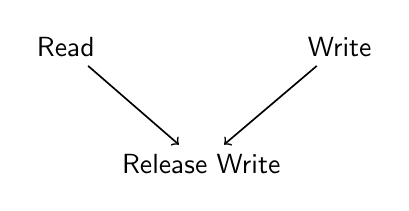
\begin{tikzpicture}[font=\sffamily]
    \node (f) at (0,0) {Release Write};
    \node (rA) [above left=1cm and 0.1cm of f]  {Read};% 2cm below, 1cm to the left (optional)
    \node (wA) [above right=1cm and 0.1cm of f] {Write};
    %\node (rB) [below left=1cm and 1cm of f]  {Read};
	%\node (wB) [below=1cm of f] {Write};
    \draw [semithick,->] (rA) -- (f);
    \draw [semithick,->] (wA) -- (f);
    %\draw [semithick,->] (f) -- (rB);
    %\draw [semithick,->] (f) -- (wB);
\end{tikzpicture}
	
\end{tabular}
\caption{Release writes and acquire reads synchronization}
\label{fig:readWrite}
\end{figure}


\subsection{Data races}
Using the \emph{happen before} relation we gave an outline of above, it is easy to get a nicer intuition of data races: an program is racy if it contains two operations on a non atomic location, one of which is a write, that are not ordered with happen before.

%We show in Figure~\ref{fig:flag} an example of a racy execution and a non racy one. In the non racy one, we use the fact that reading a value from an earlier write creates an ordering between the two operations, as well as the fact that conditionnals enforce ordering.

Note that the bits of definition of \emph{happen before} given here are in no way formal, and simply aim at giving a better intuition of the synchronization mechanisms we will study in this report.

\section{Formalizing weak memory}
We gave above some intuition of synchronization. However, this is far from enough to build any proof for a program, let alone build a verification tool. Quite a few formalizations have been proposed as a formal definition of what can happen in this context. We will here use FSL++\cite{fsl}. This separation logic formalizes a strengthening of what the C11 standard describes. The details of this strengthening are discussed in \cite{fsl}.

Let us first give an intuition of how this logic works. One further simplification imposed by this logic is that all locations are either atomic or non atomic (whereas in C++ a cast could change that).

\subsection{Atomics as exchange points}
As we explained in the previous section, we usually use atomics to protect non atomic locations from data races. Atomics are simply here to transfer some information between threads, to ensure proper synchronization, and let non atomics do the actual program work. This is for instance what we do if we build a parallel program using locks: the atomics within the locks enforce proper synchronization, and we use the rest of the variables to do all the computations we are interested in. 

FSL++ builds on this idea of atomics as mere signal senders between threads. For each atomic variable, one can define a location invariant $\mathcal{Q}: v \mapsto \mathcal{Q}(v)$. This invariant maps each value that can be read or stored in the atomic variable to some predicate. Now when writing to an atomic location a value $v$, a thread has to give up $\mathcal{Q}(v)$, whereas when it reads $v$ from this location, it gains $\mathcal{Q}(v)$. Some more rules are needed to ensure that when reading twice the same value from a location, we do not get twice the predicate. These rules are explained in more details in the parts of this report they are relevant to.

\subsection{Ownership}
We just saw that in FSL++ we use atomic locations to exchange predicates between threads, but what kind of predicates? We here introduce the notion of \emph{ownership}. When a new non atomic location $l$ is allocated by a thread, the thread get full ownership of it, noted $l^1$. This full ownership allows the thread to read or write to the location. This ownership can then be transferred to another thread through an atomic location for example. It could also be split in two (or more) parts: $l^{0.5} * l^{0.5}$. Some of this fractional permission can then be sent to another thread, while the other part of it is kept. With this partial permission, a thread can only read from the non atomic location $l$, and full permission is needed to write. As the total amount of ownership is $1$, and ownership cannot be created except when a variable is allocated, there can always be at most one thread having full permission, and if this is the case no other thread has any amount of permission. Hence we make sure that at most one thread can write to a variable at any given point, and if this is the case, no other thread can read concurrently to the variable. 

In \cite{fsl}, a notion of modality is also defined, to properly account for fences, however in this report, we never need to use those modalities, as synchronization always happen in such a way that no modality is present in the proof presented. We will hence not explain more about them here.

\subsection{Ghost states}
On top of ownership, the predicates stored in the location invariants of atomic locations can contain reference to a \emph{ghost state}. A ghost state is simply a special variable, that we use as a helper in the proof, to model some information that cannot be translated simply using ownership. When defining this special variable, we also define the domain in which it takes its values. Carefully choosing this domain allows to model complex protocols, that could not be modeled using FSL++ otherwise. In this report, we will only use one kind of ghost state domain, the entity  fractional-counting (EFC) permission structure. It was defined in \cite{gaurav}, and allows to prove with few ghost locations the examples that were studied in \cite{gaurav}.

The EFC permission structure is defined as 
\[\left(\left(\mathbb{N}_{>0} \times \mathbb{Q}_{>0} \times\{-,+\}\right) \cup\left\{(a, 0)^{+},(a, 0)^{-} | a \in \mathbb{N}\right\}, \oplus,(0,0)^{+},(0,0)^{-}\right)\]
with the partial commutative and associative operation $\oplus$ defined as 
\[\begin{array}{r}
{(c, d)^{+} \oplus(a, b)^{-} :=(a, b)^{-} \oplus(c, d)^{+} :=
\left\{\begin{array}{cl}
&{\text { if } a-c }{\geq 0 \text { and }} \\ 

{(a-c, b-d)^{-}} & {b-d }{\geq 0 \text { and }} 
\\ &({a-c}  {=0 \Rightarrow} {b-d}  {=0})\\

{\text { undefined }}&{{otherwise }}
\end{array}\right.} \\ 
\end{array}
\]
		
\[(a, b)^{+} \oplus(c, d)^{+} :=(a+c, b+d)\]

\[(a, b)^{-} \oplus(c, d)^{-} :=\text {undefined }\]

The idea of this permission structure is to have a single source permission $(c, s)^-$, and some amount of tokens $(1, s)^+$. The operation $\oplus$ being undefined for two values with $-$ ensures that there can only be one source permission. This permission structure corresponds to the intuition one can have of an atomic location $l$ protecting a non atomic location $d$. We can have in the location invariant of $l$ the source permission, while threads that change the value of the atomic location gain or give up some tokens. The tokens are usually of the form $(1, s)^+$: they are hence unsplitable (because of the 1), and $s$ usually specifies the amount of permission the thread owns to $d$. For instance a token $(1, 1)^+$ specifies write permission. As $\oplus$ is not defined for some values, a thread owning $(1, 1)^+$ ensures that the source must be $(c, 1)^-$, recording the fact that there is no permission left.

We explained above the idea of the tokens being related to an amount of permission. The tokens themselves do not give any permission to a thread. By defining carefully the invariant for $l$, we can make sure that a thread can only gain permission at the same time as gaining a token. This can then be used in the proof, by reasoning on the values of tokens and sources, to prove that the program respects the invariant.

\subsection{Token-based reasoning in Viper}
In \cite{pascal}, Wiesman et al. abstracted some of the complexity of FSL++ and the EFC permission structure, to be able to implement a tool that could be used in Viper, and automate as much as possible of the reasoning for concurrent C++ programs. Token based reasoning unifies the permission to a location $d^s$, and the token $(1, s)^+$, into a new kind of token. It also removes the exact amount of the permission $s$, replacing it with either \emph{write, read} or \emph{none}. The possible tokes are hence 
\[\texttt { Tok }(\text {loc}, n, \tau) \text { where } n \in \mathbb{N}_{>0} \text { and } \tau \in\{ {none, read, write}\}\]
and the source is now 
\[\texttt{Src}(l o c, n, \tau) \text { where } n \in \mathbb{N} \geq 0, \text { and } \tau \in\{ {none, read, write}\}\]

This allows for simpler automation rules, at the price of some approximation, as we will see in Section~\ref{sec1}.


%djksljflkdsjfldks

%fetch and add  + cas - false rules (fig 3 et 4 de gaurav p/13)

\chapter{Ease of use limitations of the EFC ghost location and tokens}
In this chapter, we will use the Folly library reader writer lock \cite{follyRW} to explicit some limitations of the EFC monoid defined in \cite{gaurav} and the token-based reasoning developped in \cite{pascal}. While, as we will see, those limitations can easily be overcome using some simple tricks, they make reasoning less intuitive, and those tools harder to use.

\section{The Folly reader-writer spinlock}
The Folly reader-writer lock is used to allow multiple threads to access concurrently a shared resource \emph{res}, with either reader or writer priviledge. This lock allows multiple reader threads to access \emph{res} concurrently, but makes sure that if a thread has write access, all other threads are forbidden from reading or writing to it. The (simplified) implementation of this lock is shown in Figure~\ref{fig:follyRWL}. This implementation is taken from \cite{gaurav}.

The idea of the implementation is quite simple. It uses an atomic location \emph{bits}. The least significant bit of \emph{bits} (which we will denote as \emph{lsb(bits)})indicates wether or not there is currently a thread with write access, while \emph{bits / 4} indicates the number of threads currently having or attempting to have a read access. When a thread wanting a read access to \emph{res} calls the function \texttt{try\_lock\_shared()}, it first increments \emph{bits} by 4. Then it checks for the value \emph{lsb(bits)} had when it was incremented by 4. If it is null, then there is currently no writer thread. The call to \texttt{try\_lock\_shared} succeeded, and the calling thread got read access. If it is not null, the thread decrements \emph{bits} by 4 and the call failed: no access is gained. To release a reader lock, a thread simply decrements the \emph{bits} variable by 4, using the \texttt{unlock shared function}. To get a write-lock, a thread calls \texttt{try\_lock}, which simply atomically checks if \emph{bits} is 0 (that is to say there is no reader thread or thread currently attempting to get read access), and if so changes it to 1. Finally, to release a writer-lock, \emph{lsb(bits)} is simply set to 0.

\section{Proof using the EFC permission structure}
As explained in more detail in Chapter~\ref{ch:background}, the EFC permission structure is based on the idea of giving entities, containing some amount of permission and a token, to each thread that asks for it. We then record the number of tokens, and the total amount of permission that were distributed, to be able to track if full permission is available or not. 

Hence, when trying to prove this implementation to be correct using the EFC permission structure, the first idea that comes to mind is to use only one ghost state in the invariant, quantifying how many permissions, and which amount of permission were given away. This leads to the following invariant:

$$\begin{aligned} \mathcal{Q}^{EFC}(v) :=& \operatorname{let} n=\left\lfloor\frac{v}{4}\right\rfloor + lsb(v), w=\operatorname{lsb}(v), \text { in } \\ & \exists s \in \mathbb{Q} \cap[0,1] \cdot v \geq 0 \wedge (w=1 \Leftrightarrow s=1) \wedge \\ & resource(\mathrm{bits})^{1-s} * \ghost{\lambda :(n, s)^{-}}
\end{aligned} $$

while the read and write permission are represented by:
$$\rPerm = \exists q \in (0, 1].\ress{q}* \ghost{\lambda : (1, q)^+}$$

$$\wPerm = \ress{1} * \ghost{\lambda:(1, 1)^+}$$

Here a read permission is tracked with a token and some non null amount of permission $\ghost{\lambda :(1, q)^+}$, while a write permission corresponds to the full permission 1: $\ghost{\lambda:(1, 1)^+}$. The source $\ghost{\lambda :(n, s)^{-}}$ in the invariant tracks the number $n$ of tokens that were given away, as well as the amount of permission $s$ that was given along. Finally, in the \texttt{try\_lock\_shared} function, a thread may increment the location \emph{bits} without actually gaining any permission, if there is already a writer thread along. In this case, the thread temporarily gets an empty token, with no permission $\ghost{\lambda:(1, 0)^+}$.  We show in Figure~\ref{fig:specRWFolly} the function specifications we would like to prove. 

Note that here the tokens represented by the ghost location do not hold any permission by themsleves, they are simply used to track the permission that is actually transmitted through $\ress{q}$.

\begin{figure}
		$$\Uperm \texttt{bool try\_lock\_shared()}\{y. (y ? \rPerm : \emp)\}$$
\[
\left\{\begin{array}{l}\Uperm* \\ {\rPerm}\end{array}\right\}
\texttt{void unlock\_shared()} \{\emp\} \]


$$\{\Uperm\}\texttt{bool try\_lock()} \{y. (y ? \wPerm : \Uperm)\}$$


\[
\left\{\begin{array}{l}\Uperm* \\ \wPerm* \\ (\texttt{getRead} ? \\ \ghost{\lambda: (1, 0)^+} : \\ \emp) \end{array}\right\}
\texttt{void unlock(bool getRead)}
\left\{\begin{array}{l}(\texttt{getRead} ? \\ \rPerm : \emp) \end{array}\right\} \]

\[
\left\{\begin{array}{l}\Uperm* \\ \wPerm* \end{array}\right\}
\texttt{void unlock\_and\_lock()}
\{\rPerm\} \]
\caption{Specifications of the lock functions}
\label{fig:specRWFolly}
\end{figure}

While this invariant and specifications seem quite straightforward, they are not sufficient to prove correctness of the \texttt{unlock\_shared} function. Let us go through the proof.

We use the fetch-and-add rule shown in Figure~\ref{fig:faaddRule}, using $\mathcal{P}_{\text{send}} = \rPerm$ and $\mathcal{P}_{\text{keep}} = \emp$. It is hence sufficient to show that for all values  $v \geq 0$, we have that 

\[
\begin{array}{l}
\{\Uperm * \rPerm\} \\
\texttt{CAS}^{\text{rel}}(\texttt{bits}, v, v - 4) \\
\{y. (y = v \land \emp) \lor (y \neq v \land \Uperm * \rPerm)\}
\end{array}\]

To do so, we use disjunction.
If $v < 4$ and $\texttt{lsb}(v) = 0$, we have that $\mathcal{Q}(v) \Rightarrow \efcm{0}{0} * \text{true}$ (we here use that $(0, x)$ is in the domain of the EFC permission structure if and only if $x = 0$). We hence have that $\mathcal{Q}(v) * \efcp{1}{0} \Rightarrow \text{false}$, as $\efcp{1}{0} \oplus \efcm{0}{0}$ is undefined. The \textsc{cas}-$\bot$ rule shown in Figure~\ref{fig:} then allows us to conclude this case.

The second case is $v < 4$ and $\texttt{lsb}(v) = 1$. In this case we have that $\mathcal{Q}(v) \Rightarrow \efcm{1}{1}$. We hence have again that  $\mathcal{Q}(v) * \efcp{1}{0} \Rightarrow \text{false}$, as $\efcp{1}{0} \oplus \efcm{1}{1}$ is undefined. We then use the \textsc{cas}-$\bot$ rule again.

The proof then fails for the case $v \ge 4$ and $\texttt{lsb}(v) = 1$. In this case, we would like to use again the \textsc{cas}-$\bot$ rule: in our implementation, this can never happen, as we cannot at the same time have given a write permission (as denoted by $\texttt{lsb}(v) = 1$) and a read permission (currently owned by the thread calling \texttt{unlock\_shared}). However, the invariant fails to capture this idea. The only information we can get from it here is that the amount of permission that was given away in total is $1$. For instance an invariant containing the ghost location $\ghost{\lambda:(3, 1)^-}$ could denote either that 3 readers each got permission 1/3 to the resource, or 1 writer got full permission, and two threads are trying to get reader access (and are currently running the \texttt{try\_lock\_shared} function). We could not express using only one ghost locationt that the first case cannot happen.

While this example shows that the EFC permission structure is a bit less expressive than we can think it to be at first sight, this proof can easily be made to work using one extra ghost location, as is done in \cite{gaurav}. This extra ghost location captures exactly the information we showed was lacking before: is there currently a thread owning write permission?

It is interesting to note that this problem is not encountered in the Rust Atomic Reference Counter proof using an EFC ghost state developped in \cite{gaurav}. This is simply because in this case, we only ever give away read accesses. It can hence be hardcoded in the invariant that the amount of permission given away is always strictly less than 1.



\section{Proof using token-based reasoning}
We saw in the previous section how the EFC permission structure is weaker in practice than what our intuition dictates. While this limitation can easilly be overcome, it is at the price of slightly less intuitive proofs. We will see here that the token-based reasoning developped in \cite{pascal} is itself weaker than the EFC permission structure it was based on.

If we were to straightforwardly translate the proof developped in the previous section using the tokens defined in \cite{pascal}, we would get the invariant and read and write permissions shown in Figure~\ref{fig:invToksRWFolly}.

\begin{figure}
$$\begin{aligned} \mathcal{Q}^{EFC}(v) :=& \operatorname{let} n=\left\lfloor\frac{v}{4}\right\rfloor + lsb(v), w=\operatorname{lsb}(v), \text { in } \\ & v \geq 0 \wedge (w = 1 ? \texttt{Src}(res, n, write) : \texttt{Src}(res, n, read))
\end{aligned} $$

$$\rPerm = \texttt{Tok}(res, 1, read)$$

$$\wPerm = \texttt{Tok}(res, 1, write)$$
		\caption{Simple invariant and Read-Write permissions for the Folly Reader-Writer Spinlock}
		\label{fig:invToksRWFolly}
\end{figure}

Now, in the \texttt{unlock\_shared} function, we would like to prove that we cannot read $v < 4$ from the location \texttt{bits}. Here we cannot do it, as the token we own is not incompatible with the location invariant. Reading $v < 4$ and $lsb(v) = 1$ from \texttt{bits} yields $\texttt{Src}(res, 1, write)$. Using the \textsc{any-src-read-tok}, we could then combine the source with our read token to get $\texttt{Src}(res, 0, read)$, which using the \textsc{all-tokens-a} yields $\texttt{Src}(res, 0, write)$. We could not reach any contradiction here.

This is because the tokens allow for "downgrading" of a token, from write to read permission. Hence is could happen that a threads gets write permission, downgrades it to read permission, then gives back this permission. The source then has to be able to reconstruct from the number of tokens it has wether or not it now owns full permission or not. This could not happen using the EFC ghost state directly as such a downgrading of tokens is not possible: the amount of permission $q$ contained in a ghost location $\ghost{\lambda : (1, q)}$ cannot be made lower without further dividing the token.

We here see that the proof fails earlier than when using the EFC permission structure, showing a small difference between the two reasonings. This can again be easilly fixed, by making the proof a little less straightforward. We can for instance use the idea developped in \cite{pascal} for the Rust Atomic Reference Counter proof: defining a different amount of tokens for read an write permissions. This outcome can then be forbidden. By giving 3 tokens for read permission and 2 for write, we would reach a contradiction by trying to combine  $\texttt{Src}(res, 2, write)$ and $\texttt{Tok}(res, 3, read)$, using rule \textsc{too-many-tokens}. This trick allows us to get as far in the proof as we did using the EFC ghost location, but we then get stuck in the next step: proving that $v \geq 4$ and $lsb(v) = 1$ is not possible. This is what we would expect: the tokens are not more powerful than the EFC ghost location.


\chapter{Limitations of FSL++}
In the previous section, we showed some limitations of the EFC permission structure and token-based reasoning. However, those limitations could be overcome, though they made proofs less intuitive and hence harder to write. In this section, we will develop on some limitations of FSL++. Those limitations seem more fundamental, as we could not find ways to overcome them, and at least one would require an extension to the FSL++ logic. We will develop those limitations using two examples, from the glibc and Folly libraries.

\section{glibc Reader-Writer Lock}
We will first focus on the glibc Reader-Writer lock \cite{glibcRW}. As we will see in Section~\ref{subsec:glibcRWPb}, it cannot be proven in FSL++ for a deceptively simple reason. We will still describe it in details, as its synchronization mechanism is quite interesting, and shows how a slightly different implementation can make for different (or impossible in this case) proofs.

\subsection{Implementation}
The implementation of this lock is shown in Appendix~\ref{app:glibc}. This implementation was heavily simplified from the original one.% In particular, futexes (special variables used to wake-up a thread when an event occurs) which where used to prevent extra spining where removed. While they are important to make the code more efficient, they are not part of the synchronization mechanisms used to ensure correctness of this lock.

\begin{figure}
		\begin{center}
		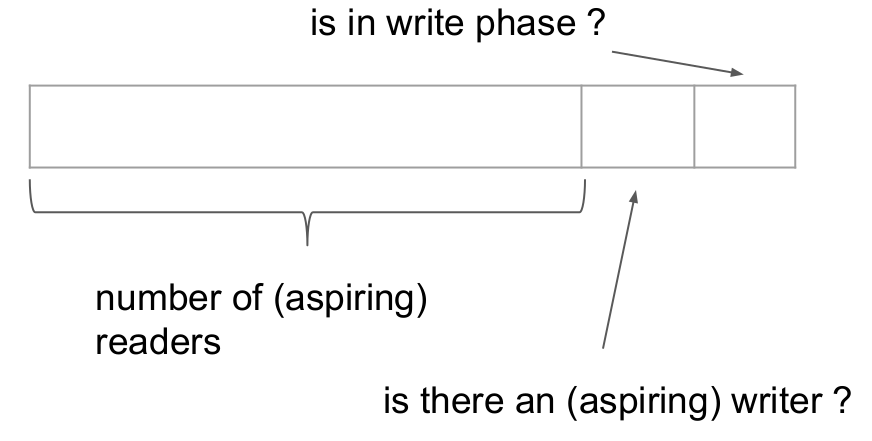
\includegraphics[width=\linewidth]{schemaglibc.png}
		%\caption{glibc reader-writer lock}
		\end{center}
		\caption{glibc reader-writer lock}
		\label{schemaglibc}
\end{figure}

Just as the Folly reader-writer lock, this lock offers four main functions: \texttt{readLock} (equivalent of \texttt{lock\_shared}), \texttt{readUnlock} (\texttt{unlock\_shared}), \texttt{writeLock} (\texttt{lock}) and \texttt{writeUnlock} (\texttt{unlock}).

This implementation uses a single atomic location \texttt{\_\_readers}, used similarly as the location \texttt{bits} in the Folly reader writer lock. This location is used as shown in Figure~\ref{schemaglibc}. The least significant bit is used to denote if the lock is in read or write phase. As can be expected, if it is in read phase, only reader access can be granted, while if it is in write phase, only writer access can be granted. The second least significant bit tells whether or not there is currently a thread asking for or having write access. Finally, \texttt{\_\_readers} $/ 8$ gives us the number of threads currently owning reader access or requesting it. For easier reading, we use the following denotation for the value of \texttt{readers\_\_}: $\mathtt{readers\_\_} / 8 | lsb(\mathtt{readers\_\_ }/ 2) | lsb(\mathtt{readers\_\_})$. For instance, $2|1|1$ corresponds to \texttt{readers\_\_} $=19$, which means the lock is currently in write phase, and that one thread owns a write access, while two threads are requesting a read access. If it were to contain $2 | 0 | 1$, it means it is still in write mode, but no thread owns write access to it. The implementation makes sure that in this case one of the threads requesting read access will change the least significant bit to $0$, allowing for read access.

Each of the functions then uses appropriate synchronization mechanisms to ensure the value of \texttt{\_\_readers} accurately reflects the permissions threads hold to the protected location, as well as proper synchronization when taking or releasing the lock. A more detailed explanation of the lock implementation can be found in the Appendix~\ref{app:glibc}. The synchronization mechanisms are quite complex, and not necessary to understand the following.

We will here only focus on a further simplification of the \texttt{readerLock} function which is sufficient to show the different mechanisms we are interested in. 
%We simply remove loops and replace them with \texttt{if} statements. Note that note only the call to lock can now fail, but it may also put the lock in an inconsistent state (as it may increment the number of readers, and never decrement it). However, we are here only interested in successfull executions of this simplification. 
This simple code is shown in Figure~\ref{fig:codeglibc}.

\begin{figure}
		\begin{lstlisting}
Constants:
WRLOCKED = 2
WRPHASE = 1

int readLock(){
	int r = fetchAndAdd_Acq(__readers, 8) + 8
	if(r & WRPHASE == 0)
		return 0
	while(r & WRPHASE != 0 && r & WRLOCKED == 0){...}

	while(Load_Acq(__readers) & WRPHASE == 1){;}
}

	\end{lstlisting}
	\caption{\texttt{readLock function}}
	\label{fig:codeglibc}
\end{figure}
In the rest of this section, we will only use two executions scenarios to support our reasoning. They are shown in Figure~\ref{fig:scen1} and Figure~\ref{fig:scen2}. The first one is the most straightforward: there is only one thread trying to get the lock. It calls \texttt{readLock()}. The \texttt{fetchAndAdd} occurs, increasing the number of potential reader threads by 1. We then check if the least significant bit (corresponding to \texttt{WRITEPHASE}) is set to 0. As it is the case, the function returns: Thread 1 now has a read lock. In the second scenario, Thread 1 holds a write lock when Thread 2 calls the \texttt{readLock} function. Hence after the \texttt{fetchAndAdd}, neither the \texttt{if} condition nor the following \texttt{while} condition succeed. Thread 1 then releases the lock. The condition of the final \texttt{while} is then satisfied. The function returns and Thread 2 now holds a read lock.

We see here that the calling thread can get read access to the resource in two distinct points \footnote{There is actually a third one in the elided code, but it is not relevant to our discussion here}. This is quite different from the Folly reader-writer spinlock implementation, where the access was granted by the \texttt{fetchAndAdd} operation only. If the lock was already taken, the function would cancel this add (by subtracting the same value), and fail. We will see now how this proves to be a problem when formalizing this lock in FSL++.


\begin{figure}
\begin{tabular}{c||c}
	\texttt{\_\_readers} & Thread 1\\
	0 | 0 | 0 & \\
	 &   \texttt{fetchAndAdd\_(\_\_readers)} \\
	1 | 0 | 0 & \\
	 & \texttt{if(r \& WRPHASE == 0) } \\
	& \texttt{return 0 } \\
	&  Read lock succeeds!
\end{tabular}

		\caption{First \texttt{readLock()} execution scenario}
		\label{fig:scen1}
		%\caption{First \texttt{readLock()} execution scenario}
\end{figure}
\begin{figure}
\begin{tabular}{c||c|c}
	\texttt{\_\_readers} & Thread 1 & Thread 2 \\
	0 | 0 | 0 & & \\
	 & \texttt{writeLock()} & \\
	0 | 1 | 1 &   & \\
	 &   & \texttt{fetchAndAdd\_(\_\_readers)} \\
	1 | 1 | 1 & & \\
		& & \texttt{if(r \& WRPHASE == 0) ...} \\
		& & \texttt{while(r \& WRPHASE != 0 ...} \\
	 & \texttt{writeUnlock()} & \\
		1 | 0 | 0 & & \\
		& & \texttt{Load\_Acq(\_\_readers) \& WRPHASE} \\
		& & Read lock succeeds!
\end{tabular}

		\caption{Second \texttt{readLock()} execution scenario}
		\label{fig:scen2}
		%\caption{Second \texttt{readLock()} execution scenario}
\end{figure}


		\subsection{Read-Modify-Write and Load}
	\label{subsec:glibcRWPb}
As we saw in the two executions scenarios described above, read permission can be given either by a fetch-and-add, or by a subsequent load. However, when looking into the proof rules of FSL++, none of them allow for gaining resources from a single atomic location both using a Load and a fetch-and-add. When looking further into it becomes quite clear why such a rule would be quite difficult to implement.

In FSL++, atomic locations are used to transfer ownership (here to the resources protected by the lock) between threads. It does so by using a location invariant $\mathcal{Q}$ which for each value $v$ gives the ownership corresponding to this value. Then when writing value $v$ to the atomic location, a thread has to give up the assertion $\mathcal{Q}(v)$, and when reading value $v$, a thread gains this assertion. However this simplistic idea is not sufficient: it could happen that Thread 1 writes $v$, giving up $\mathcal{Q}(v)$, then Thread 2, reads $v$, gaining $\mathcal{Q}(v)$, then Thread 3 reads as well $v$, gaining $\mathcal{Q}(v)$. Here, the assertion $\mathcal{Q}(v)$ has been duplicated, which is clearly unsound \footnote{For instance if $\mathcal{Q}(v) = \ress{1}$, this would lead to total permission access to a location striclty greater than 1.}. To forbid this outcome, FSL++ introduces the assertions $\acqPerm$ and $\relPerm$. When a new variable is created, the corresponding permissions $\{\acqPerm * \relPerm\}$ are created. $\relPerm$ can then be freely duplicated, whereas the $\acqPerm$ can only be transmitted, making sure only one thread is allowed to get ownership from the location (all threads can read from the location, but they will get no ownership from it). 

Now for read-modify-write operations, that is to say operations that read and write atomically to a variable, the situation is different. As the value of the variable is read and changed in one atomic operation, the duplicating problem does not occur anymore. If thread 1 does a fetch-and-add and reads value $v$, it gets $\mathcal{Q}(v)$, and gives $\mathcal{Q}(v + 1)$. Hence if another thread then does another fetch-and-add there is no risk of inadvertently getting twice the same permission. Hence we can be more permissive here, allowing multiple threads to perform read-modify-writes to the same location, and all gaining ownership. To allow for this, when a new variable is created, FSL++ offers a choice between $\relPerm * \acqPerm$ or $\relPerm * \rmwPerm$. The latter is then freely duplicable and can be transmitted to all threads requiring it. There is however no rule that would allow to have both $\operatorname{\mathsf{Acq}}(\ell, \mathcal{Q}_1)$and $\operatorname{\mathsf{RMWAcq}}(\ell, \mathcal{Q}_2)$ for the same location, with $\mathcal{Q}_1$ not empty.

A new logic rule that would allow for this would be difficult to design, as it would have to take into account the duplicability of $\rmwPerm$ and non duplicability of $\acqPerm$.

	\subsection{Separation of tokens and permission}
We saw in the previous section how FSL++ rules do not allow for a proof of the glibc reader-writer lock. Another interesting point of this lock when thinking in terms of the EFC permission structure, is that it separates tokens from permission. In the second scenario Figure~\ref{fig:scen2}, thread 2 increments the number of readers with the fetch-and-add, but only gets permission with the load in the second while. This would hence make counting the number of permissions given away (as recorded by \texttt{\_\_readers / 8}) difficult to link with the amount of permission given (done in the load here).

\section{Folly One Producer One Consumer Queue}
\label{sec:2b}
We saw in the previous section that we could not use FSL++ to prove strong results about the glibc reader-writer lock, because it lacked support for both read modify writes and loads to the same variable. We will now focus on a different example, using only store/load, to avoid encountering this shortcoming again.

This new example is the Folly ProducerConsumerQueue \cite{queue}, a concurrent fixed size queue. It allows for exactly one producer thread, and one consumer thread. The queue is implemented using a circular buffer, as well as release stores and acquire loads for synchronization. The full code, including some extra functions that we will not discuss can be found in Appendix~\ref{app:queue}. We will here use the simplification of the code shown in Figure~\ref{fig:queueCyclic}.

An object \texttt{Queue} contains four fields: its size, an array \texttt{records} of size \texttt{size\_}, and two atomic indices \texttt{readIndex, writeIndex}. When creating the object, both indices are set to $0$. The queue offers two main functions: \texttt{write} which takes an argument and adds it to the queue if it is not full, and \texttt{read} which returns the last element if the queue is not empty. 

Note here that in spite of its name, the read function requires full ownership to the array slot it is reading, as it deletes it when returning it. This means that the producer and consumer threads need to transfer full ownership between one another during those function calls.

\begin{figure}
\begin{lstlisting}
bool write(toWrite){
	int curWrite = load_rlx(writeIndex)
	int nextWrite = (curWrite + 1) % size_
	int curRead = load_acq(readIndex)
	if(nextWrite != curRead){
		records[curWrite] = toWrite
		store_rel(writeIndex, nextWrite)
		return true
	}
	return false
}
bool read(&valRead){
	int curRead = load_rlx(readIndex)
	int nextRead = (curRead + 1) % size_
	int curWrite = load_acq(writeIndex)
	if(curRead == curWrite)
		return false
	valRead = records[curRead]
	delete records[curRead]
	store_rel(readIndex, nextRead)
	return true
}

\end{lstlisting}
		\caption{Simplified code for the Folly one producer one consumer queue}
		\label{fig:queueCyclic}
\end{figure}

This code is quite simple. Let us focus on the \texttt{read} function in more detail. This function first reads the current read index. Note that this read is relaxed. It is used here only to have a nicer interface for the function: as there is only one consumer thread, this thread could remember the \texttt{readIndex} value from one call to another, and pass it as an argument to the function, without fundamentally changing the function. We then compute the position of the next slot in the array (which we use as a circular buffer hence the need for \%). The first synchronization then comes in: the value of \texttt{writeIndex} is read with an \texttt{acquire} synchronization. This synchronization ensures that all reads or writes that come after will not be re-ordered before. We then check whether the queue is empty. If not, we store the current record in the reference that was passed as argument to the function, then delete the record. Finally, we use a release store to update the value of \texttt{readIndex}.

\begin{figure}
		\begin{center}
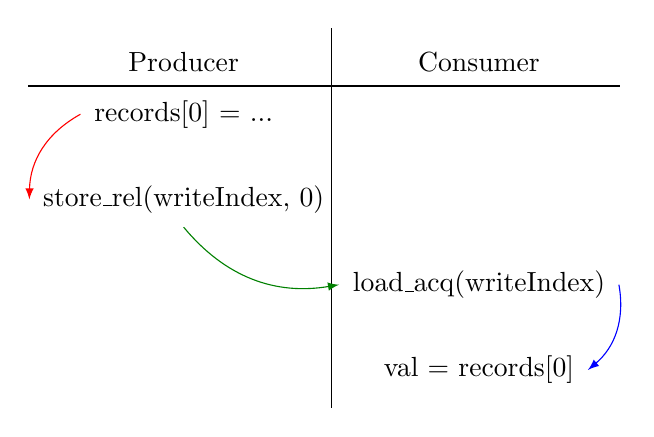
\begin{tikzpicture}%
  \node[%
  matrix of nodes,%
  inner xsep=0pt,% <- code added
  every node/.append style={%
    draw=white,
    inner xsep=5pt,
    inner ysep=5pt,
    outer sep=0pt,
  },
  row sep=0pt,
  column sep=0pt
  ] (M) {
    Producer & Consumer \\
	records[0] = ... & {} \\
	{} & {}\\
	store\_rel(writeIndex, 0) & {} \\
	{} & {}\\
	{} & load\_acq(writeIndex) \\
	{} & {}\\
	{} & val = records[0] \\
  };
% horizontal lines
  \draw[black]({$(M-1-1)!.5!(M-1-2)$} |- M.north) -- ({$(M-1-1)!.5!(M-1-2)$} |- M.south);
  %\draw[orange!80!black]({$(M-1-2)!.5!(M-1-3)$} |- M.north) --({$(M-1-2)!.5!(M-1-3)$} |- M.south);
% vertical lines
    \node[fit=(M-2-1) (M-2-2),inner sep=0pt] (R2) {};
    \draw[black] (R2.north -| M.west) -- (R2.north -| M.east);
%hb
		\draw[red,->,>=latex](M-2-1.west) to[bend right] (M-4-1.west);
		\draw[green!50!black,->,>=latex](M-4-1.south) to[bend right] (M-6-2.west);
		\draw[blue,->,>=latex](M-6-2.east) to[bend left] (M-8-2.east);
\end{tikzpicture}
\end{center}
%\label{fig:synchQueue}
\caption{Synchronization in the Folly one producer one consumer queue}

\label{fig:synchQueue}
\end{figure}


To better explain the synchronization ensuring that there is no data race on \texttt{records}, we focus on a simple scenario: we start from an empty queue, the producer thread then stores a value in \texttt{records}, and the consumer thread then reads it. Part of this scenario is shown in Figure~\ref{fig:synchQueue}. The release store to \texttt{writeIndex} ensures that any memory operation happening before it will be visible to other threads when they see the value released. In particular, any thread reading the new value of \texttt{writeIndex} will have the proper value stored in \texttt{records[0]}. This is materialized by the red arrow. Then the acquire load ensures that any memory operation after it will not be re-ordered. In particular, reading in \texttt{records[0]} will happen after this value was read, as shown by the blue arrow. Finally, as in this scenario the load acquire reads the value from the previous release store, we have an ordering between the two shown by the green arrow. There is hence a proper ordering between the write access to \texttt{records[0]} by the producer thread and the read access to it by the reader thread: data races are avoided.

\subsection{Re-using values for location invariants}
We saw in the previous section about the glibc reader-writer lock the need for $\acqPerm$ predicates, to ensure ownership could not be duplicated, for instance by two threads reading to the same value. The restrictions on this predicate are actually even stronger than what we developed there. The rule for a read\footnote{This rule is slightly simplified, some conditions are required on $\mathcal{Q}$.} in FSL++ is 
\[
		\{\acqPerm * \mathsf{Init(\ell)}\} \mathtt{load\_acq}(\ell) \{v.\mathsf{Acq}(\ell, \mathcal{Q}[v:=\mathsf{emp}]) * \mathcal{Q}(v)\}
\]

Hence reading value $v$ from a location $\ell$ uses our permission to do so. When the thread next reads the same value from this variable, it will not be able to gain any ownership from it. The only way we could gain ownership twice or more from reading the same value would be by splitting the $\acqPerm$ beforehand, using the following rule
\[
		\acqPermp{1} * \acqPermp{2} \equiv \mathsf{Acq}(\ell, \lambda v. \mathcal{Q}_1(v) * \mathcal{Q}_2(v))
\]

However, as noted when presenting the implementation of this queue, both the \texttt{read} and \texttt{write} function require full ownership. As full ownership cannot be split into two (or more) full ownership, we cannot apply this rule here. Besides, FSL++ does not contain any rule that would allow for strengthening the location invariant $\mathcal{Q}$ within $\acqPerm$. This means that when the location invariant in an acquire permission is set to \texttt{emp} for some value $v$, it can never be made non-empty again. 

So, if we were to prove the \texttt{read} code correct, we would need some invariant $\mathcal{Q}$, for the location \texttt{writeIndex} (as the synchronization uses this location). This invariant would need to contain full permission for the slot in the \texttt{records} array that the consumer thread can read. Now after some calls to the \texttt{read} and \texttt{write} functions, we may read the same value again from \texttt{writeIndex}, as the slots in the circular buffer are used again and again. At this point, since $\mathcal{Q}$ cannot be split while keeping full permission, it has been kept full, and $\acqPerm$ now has $\mathcal{Q}(v) = \mathsf{emp}$. We cannot gain any new ownership. This is the case no matter which location invariant $\mathcal{Q}$ we chose, as long as it contains the full ownership required by the \texttt{read} function. Hence we cannot prove this code to be correct using FSL++.

\subsection{Infinite queue}
As we have seen above, as the queue implementation uses many times the same slots in the \texttt{records} array, used as a circular buffer, we cannot prove it using FSL++. A simplification that immediately comes to mind would be to use an infinite array for \texttt{records}. The queue would not be limited anymore, and most importantly for us, slots in \texttt{records} are not re-used anymore.

Sadly, here again we were not able to use FSL++ to prove this simplified code correct. The code of the simplification is shown in Figure~\ref{fig:queueCode}. 

\begin{figure}
\begin{lstlisting}
bool write(toWrite){
	int curWrite = load_rlx(writeIndex)
	int nextWrite = (curWrite + 1)
	records[curWrite] = toWrite
	store_rel(writeIndex, nextWrite)
	return true
}
bool read(&valRead){
	int curRead = load_rlx(readIndex)
	int nextRead = (curRead + 1)
	int curWrite = load_acq(writeIndex)
	if(curRead == curWrite)
		return false
	valRead = records[curRead]
	delete records[curRead]
	store_rel(readIndex, nextRead)
	return true
}

\end{lstlisting}
		\caption{Simplified code for the Folly queue with infinite buffer}
		\label{fig:queueCode}
\end{figure}



Again, the problem lies in how we store ownership in location invariants. We denote $\mathcal{Q}$ the location invariant of \texttt{writeIndex}. When the producer thread adds a new value to the queue, it updates the value of \texttt{writeIndex}, and hence needs to give up the corresponding assertion $\mathcal{Q}(v)$. Now if the \texttt{read} function is then called, it reads \texttt{writeIndex}, and gets the corresponding $\mathcal{Q}(v)$. However, if this is not the case and \texttt{write} is called again, it gives up $\mathcal{Q}(v + 1)$. The consumer thread calling \texttt{read} will then have access to $\mathcal{Q}(v + 1)$, but has no way to access $\mathcal{Q}(v)$ again. All the ownership contained in it is lost: neither the producer nor the consumer can gain access to it again.

Here the correctness of this implementation relies on the fact that only the consumer thread can gain ownership through \texttt{writeIndex}, and this variable is always increased by $1$. Hence if the consumer thread reads $1$ then $4$ from it, it is as if it had read $2$ and $3$ as well. We were not able to model this idea using FSL++. This is not a problem when using read modify write, as in this case all intermediate states of the variable are observed by one of the threads: each write to this variable has to be preceded by a read to it.

Note that it would be tempting here to use the fact that the producer thread begins the \texttt{write} function by reading the value \texttt{writeIndex}. One could imagine that through this read the producer thread can get back the resources it previously gave up. However, remember that $\acqPerm$ containing full ownership cannot be split between two threads, as explained for the circular queue. This idea hence cannot be used here.

We are hence unable to prove this simplification of the queue to be correct. 

\chapter{Proving intertwined synchronization mechanisms}
\label{ch:serialExec}
In this chapter we will focus on a new example from the Folly library: the Serial Executor \cite{serialExec}. This example makes use of two independent synchronization mechanisms, using two atomic locations. We will show how FSL++ allows us to prove those two mechanisms almost independently. % We prove here some properties about this example using the EFC permission structure and FSL++. 
We have not proven it in the proof framework developed in \cite{pascal}, but we believe that this would be possible.

To the best of our knowledge, this is the first proof of this executor in FSL++,  as well as the only example making use of more than one synchronization mechanism.

We now describe in more details this new example. An \emph{executor} is a tool that allows a thread to delegate the execution of a task. The thread simply adds this task to the executor, and the executor guarantees that the task will be executed at some point. Depending on the type of executor, the executor may provide some extra guarantees on the execution order of the task submitted to it. The executor we all know of is the CPU scheduler: it has many tasks to execute (everything currently running on the computer) and schedules them as it sees fit.

The Folly Serial Executor is an executor that guarantes that all the tasks submitted to it will be executed serially: no two of them will be executed concurrently. %The Folly Serial Executor allows a thread to delegate the execution of a task, by simply adding this task to the executor. Depending on its characteristics, the executor will then execute this task depending on its priority, or sequentially as is the serial executor case, or any other ordering. This is quite similar to what a thread scheduler does: it is given some tasks (the threads execution), and then choses when and how to run them.
%In the case of the serial executor, the executor ensures that all the tasks that are added to it are executed sequentially. 
An example use case of such an executor would be in a server for a port. We want to make sure that no two threads try to access the same port at the same time. We can hence create a serial executor \texttt{s} dedicated to that port. Now, any thread requiring action on this port will add the task to this executor. The executor will then execute those tasks one after the other, making sure no two tasks try to write to the port at the same time.

Note that it is possible that the executor uses multiple threads to execute the tasks assigned to the serial executor. The serial executor simply guarantees that this will never be done concurrently: we will not have two threads executing some tasks from the serial executor at the same time.

Besides, a serial executor guarantees that even if it is deleted, the tasks that were added to it will be executed sequentially, as if it had not been deleted.\footnote{Unless the serial executor parent, that is the executor it delegates the tasks to is deleted.}



\section{Implementation}
A simplified implementation of the executor is shown in Figure~\ref{fig:simplSerialExec}. This code is quite different from the original, as it was originally divided among two classes, and used pointers as well as customs destructors. A code more faithful to the original can be found in Appendix~\ref{app:serialExec}. 

\begin{figure}
	\begin{lstlisting}
Executor newSerialExecutor(Executor parent){
  s = alloc();
  s.parent_ = parent;
  s.queue_ = new Queue();
  s.scheduled_ = 0;
  s.keepAliveCounter_ = 1;
  return s;
}

void add(Func func, Executor s){
	s.queue_.enqueue(func);
	s.parent_.add({this->run()});
}

void run(Executor s){ //private function
	if(fetch_add_acq(s.scheduled_, 1) > 0)
		return;
	do {
		Func func = s.queue_.dequeue();
		func();
	} while(fetch_sub_rel(s.scheduled_, 1) > 1);
}

void drop(Executor s){
	int c = fetch_sub_rel_acq(s.keepAliveCounter_, 1);
	if(c == 1)
		free(s);
}

Executor copy(Executor s){
	fetch_add_rlx(s.keepAliveCounter, 1);
	return s;
}
	\end{lstlisting}

		\caption{Simplified code for the Folly SerialExecutor}
\label{fig:simplSerialExec}
	%	\caption{Simplified code for the Folly SerialExecutor}
\end{figure}


An executor is made of four fields. The field \texttt{queue\_} is used to record the tasks that are submitted to the executor. The field \texttt{parent\_} refers to another executor: the one that is the serial executor's parent. Indeed, the serial executor is merely a middleman here. It records the tasks that are submitted to it (which we will call OT) in the queue of the \texttt{queue\_} field, and using this queue creates new tasks (NT) that it then add to its parent, another executor, not necessarily serial. Those NT tasks use the \texttt{scheduled\_} field to synchronize between one another, making sure that only one of them executes OT tasks at any point in time. The NT tasks may execute concurrently, but they make sure not to concurrently run the OT tasks.
%The field \texttt{parent\_} refers to its parent executor, the one it will delegate the tasks to. Indeed, this serial executor is merely a middleman here. It records all the tasks that are submitted to it, then transforms them into one continuous task that it submits to its parent, another executor.\footnote{There is no infinite delegation here, at some point the executor's parent will be the CPU scheduler directly.} Note that we will hence be talking about two different kinds of tasks in the following dicsussion: the ones that were submitted to the serial executor, and the new ones that the serial executor created and submitted to its parent executor. The field \texttt{queue\_} is used to record the task to be executed. The queue that is used here is a concurrent single consumer multiple producer queue. The field \texttt{scheduled\_} is used to ensure sequential execution. 
Finally the field \texttt{keepAliveCounter\_} is used to track the number of references to this executor, and deleting it when there are no references to it anymore. The \texttt{scheduled\_} and \texttt{keepAliveCounter\_} fields are atomic locations.

\subsection{Ensuring sequential execution}
Let us now describe the functions of the serial executor interface. The \texttt{add} one is quite straightforward. It adds a new task, here denoted by \texttt{func}, to the executor \texttt{s}. This is done by simply adding the task to the queue, and sending a new task to the parent executor: running the serial executor \texttt{run} function. Because the parent is an executor, it guarantees that this \texttt{run} function will be executed at some later point in time. Besides, this \texttt{run} function is private and only called by the \texttt{add} function in the serial executor class. We hence have that there will be exactly one execution of \texttt{run} for each call to \texttt{add}. 

The \texttt{run} function is the one ensuring serial execution of the tasks, using the \texttt{scheduled\_} location. To explain how it works, it helps to think about what could have been an alternative implementation of this function. We could have simply used \texttt{scheduled\_} as a flag recording whether or not there is currently a task executing. The simplified code would have been the following

\begin{lstlisting}
void run(Executor s){
	if(CAS_acq(s.scheduled_, 0, 1)){
		while(!s.queue_.empty()){
			func = s.queue.pop();
			func()
		}
		CAS_rel(s.scheduled_, 1, 0);
	}
}
\end{lstlisting}

We first try to set atomically \texttt{scheduled\_} to 1. If this succeeds, this is now the only \texttt{run()} task from the serial executor \texttt{s} that can execute NT tasks. Then as long as the queue is not empty, we keep executing one after the other all the NT tasks that were added to it. When none are left, the \texttt{run()} task releases the \texttt{scheduled\_} flag by setting it to 0. However, this function requires two calls to \texttt{queue\_} per loop execution. One checking if it is empty or not and the second popping an element\footnote{Note that here, there is no risk of having a non empty queue when the condition check is done, then its elements being removed by another thread before the \texttt{pop} is done. Indeed, as \texttt{scheduled\_} is set to one, only the current task can remove elements from the queue.}. The key remark here is that we can use scheduled to count the number of elements in the queue reliably. This is what is done in the \texttt{run} function shown in Figure~\ref{fig:simplSerialExec}.

Every time this function is called, it first increments \texttt{scheduled\_} by one. As \texttt{run} is called every time an element is added to the \texttt{queue\_} by the \texttt{add} function, \texttt{scheduled\_} records the number of elements in the queue. Now if \texttt{scheduled\_} was zero before the task incremented it, the task starts executing the tasks contained in \texttt{queue\_}. This is similar to the case where the \texttt{CAS\_acq} on \texttt{scheduled\_} succeeded in the alternative implementation discussed above. Every time a task from \texttt{queue\_} is executed, \texttt{scheduled\_} is decreased by one. As \texttt{scheduled\_} tracks the number of elements in the queue, this ensures that we never try to pop from an empty queue\footnote{This is not trivial actually, it relies on the fact that no other thread can pop from the queue, and that due to the careful of ordering of actions on \texttt{scheduled\_} and \texttt{queue\_}, after the \texttt{fetch\_sub}, \texttt{scheduled\_} is smaller or equal to the number of elements in the queue.}. When \texttt{scheduled\_} reaches 0, that is to say when the value returned by \texttt{fetch\_sub} is 1, the task terminates. As in the alternative implementation shown above, \texttt{scheduled\_} has been set back to 0, allowing another \texttt{run()} task to start executing NT tasks later.

We explained above the idea of the \texttt{run} function. Let us now develop on the precise synchronization mechanisms used. As we have seen, it is \texttt{scheduled\_} that allows execution to "pass" from one thread to another. For instance, imagine Thread 1 calls \texttt{run}. It does the first fetch and add, and sees that the former value was 0. It can hence start executing NT tasks. At some point, the fetch and sub brings \texttt{scheduled\_} back to 0. Thread 1 stops executing NT tasks. Then at some later point, Thread 2 calls \texttt{run}, and starts executing tasks. Here when Thread 2 takes over execution, we have to make sure that for any other observer thread, all the memory events done by Thread 1 as part of executing the tasks stay before all the memory actions Thread 2 will do. As Thread 1 used a fetch and sub release, we know that all events executed in Thread 1 before this fetch and sub will stay before the action that set \texttt{scheduled\_} to 0. Besides, as Thread 2 uses a fetch and add acquire, all events that are executed after this fetch and add cannot be re-ordered with it. We hence have the required synchronization:
\[
				\{\text{Tasks 1}\} 
				\xrightarrow{\text{release}} 
				\{\mathtt{scheduled\_} = 0\} 
				%\xrightarrow{\text{reads}} 
				%\{\mathtt{scheduled\_} = 1\} 
				\xrightarrow{\text{acquire}} 
				\{\text{Tasks 2}\}
		\]

where we use Tasks 1 (resp. 2) to refer to the tasks executed by Thread 1 (resp. 2).

\subsection{Ensuring proper deletion when deleting references}
The functions \texttt{drop} and \texttt{copy} ensure that when all references to a serial executor \texttt{s} are gone, it is deleted, but not before that. They do so in a fashion extremely similar to that of the Rust Atomic Reference Counter, studied in \cite{fsl}. \texttt{keepAliveCounter} tracks the number of references to the serial executor. Those references can be obtained through the \texttt{copy} function, and deleted using the \texttt{drop} function. The latter then deletes the serial executor if the reference dropped is the last one. 

The only difference between this code and the one of the Rust ARC is in the \texttt{drop} function. In the Rust ARC, the code is the following (taken from \cite{fsl})

\begin{lstlisting}
int c = fetch_sub_rel(s.keepAliveCounter_, 1);
if(c == 1){
	fence_acq;
	free(s);
}
\end{lstlisting}

For the serial executor, instead of using a fence acquire only for the last decrement, every fetch and sub contains an acquire synchronization. For all the decrements that do not yield 0, this extra synchronization does not affect the behavior we want to achieve. Finally, for the last decrement, having acquire included in the fetch and sub instead of a standalone fence does not change the synchronization provided by the function\footnote{In practice, there is a slight difference: a fence acquire prevents re-ordering of any read before it with any read or write after it, whereas a load acquire only forbids re-ordering between the load itself and any subsequent read or write.}.

For a more in depth explanation of the synchronization mechanisms at play here, refer to \cite{fsl}.

%The synchronization mechanism is quite simple. When acquiring a copy, we use an acquire synchronization, ensuring all events that happened

\section{Properties of the \texttt{SerialExecutor}}
We explained above the implementation of the serial executor. We will here detail the few properties we set out to prove about this code

The first property we want to show about this code, is that the \texttt{Serial\-Executor} is indeed serial, that is to say all functions passed to it through \texttt{add} are executed sequentially, and never concurrently. As we are only interested in the synchronization mechanism here, we model this using the following simplification. We consider one non-atomic location \texttt{protected}, and consider that all functions passed to \texttt{add} need full ownership of this location for their execution, and nothing else. We hence have to show that when they are run, they are in a thread that does own this permission. The code with this simplification is shown in Figure~\ref{fig:serialExecCP}. Let us now explain why proving this simplification correct ensures non concurrent execution of the tasks. 

If we manage to prove this simplification correct, we will have proven that there is no data race on the non atomic location \texttt{protected\_}. This means, by definition of a data race as given in Section~\ref{ch:background}, that all memory operations on \texttt{protected\_} are ordered by the happen-before relation, that is to say they are all executed serially, and not concurrently. This would then allow us to conclude that the synchronization in the \texttt{run} function is enough to ensure ordering of the all operations executed within the repeat loop: setting \texttt{protected\_} to some value \texttt{a}. If we were to replace this operation by any function execution, as is the case in the original Serial Executor code, we keep this property on ordering: the functions submitted to the Serial Executor are all executed serially. 

\paragraph{Note:} One could think that proving the simplified code correct only shows that the Serial Executor provides serial execution of the write memory operations submitted to it, and not necessarily read operations. Indeed, we mentioned in Section~\ref{ch:background} that the release and acquire fences provide different ordering constraints to read and write operations. However, in the \texttt{run} function, the only synchronization operations are a release fetch and sub and an acquire fetch and add. Both of those operations do not discriminate between read and writes in the synchronization they provide, as shown in Figure~\ref{fig:readWrite}. Proving ordering of the write operations is hence enough to conclude on ordering of all memory operations, read and write alike.
\newline
\newline
The second property we are interested in is a proper use of the queue: we need to make sure that at any point there is at most one consumer, while there can be many producers. To model this, we introduce two abstract predicates $\consQ$ and $\prodQ$. They are governed by the following properties:
\begin{equation}
		\frac{}{\{\mathsf{emp}\} \texttt{q = new Queue()} \{\mathsf{Consumer}(\texttt{q}) * \mathsf{Producer}(\texttt{q})\}} 
		\tag{\textsc{new queue}} 
		\label{eq:nQ}
\end{equation}
\begin{equation}
		\mathsf{Producer}(\texttt{q}) \iff \mathsf{Producer}(\texttt{q}) * \mathsf{Producer}(\texttt{q})
		\tag{\textsc{producer duplication}} 
		\label{eq:prodDup}
\end{equation}
\begin{equation}
		\frac{}{\{\mathsf{\consQ}\} \texttt{q.dequeue()} \{y.\consQ\}} 
\tag{\textsc{Dequeue}} 
\label{eq:dQ}
\end{equation}

\begin{equation}
		\frac{}{\{\mathsf{\prodQ}\} \texttt{q.enqueue(a)} \{\prodQ\}} 
\tag{\textsc{Enqueue}} 
\label{eq:eQ}
\end{equation}
The \eqref{eq:nQ} allows us to create a new queue, and creates permission for a consumer and a producer. The \eqref{eq:prodDup} equivalence allows us to duplicate the producer permission, allowing mutliple threads to add to the queue. \eqref{eq:dQ} and \eqref{eq:eQ} simply encode that a thread con only enqueue (resp. dequeue) an element from the queue if it owns the $\prodQ$ (resp. $\consQ$) predicate. Those two predicates should be thought of as some placeholders, that could be replaced with more precise predicates defining the behavior of a single consumer multiple producers queue.

Finally we want to prove that the \texttt{keepAliveCounter} works as expected, that is to say like the Rust Atomic Reference Counter. The specification is quite simple: the deallocation of the executor \texttt{s} is not done until all threads are done with using the fields of \texttt{s} that are deallocated. However, note that the specification of the \texttt{SerialExecutor} requires that even if it is deleted, all the tasks submitted to it will still be executed with the same guarantees. %Besides, in the original code the field \texttt{protected\_} of the \texttt{SerialExecutor} is not deleted upon deallocation of the executor. 
We can rephrase this property about the \texttt{keepAliveCounter} more precisely as: no read to the \texttt{parent\_} field of the executor should race with the deallocation of this executor.

Some other properties could be proven on this code, for instance the fact that we never try to get an element from the empty queue. However, this would require first defining and proving the properties of a single consumer, multiple producer queue.


\section{Formalizing the specifications}

To produce a formal proof of the properties described above, we need to rewrite again the code of the serial executor, using only language constructs allowed in FSL++. The main change is the use of a \texttt{protected} non atomic variable to model the ressources the serial executor protects. Instead of pushing tasks \texttt{func} to the queue, we now push some integer value, and executing a task is simply assigning this value to the \texttt{protected} field. We also replace the \texttt{do ... while} loop with a \texttt{repeat}, that repeats its body until it returns a non-zero value. Finally, the \texttt{drop} function now returns the value it read from \texttt{keepAliveCounter\_}, so that we can have a more precise specification of this function. The resulting simplified code is shown in Figure~\ref{fig:serialExecCP}.

\begin{figure}
	\begin{lstlisting}
Executor newSerialExecutor(Executor parent, Ress protected){
  s = alloc();
  s.protected_ = protected;
  s.parent_ = parent;
  s.queue_ = new Queue();
  Store_Rel(s.scheduled_, 0);
  Store_Rlx(s.keepAliveCounter_, 1);
  return s;
}

void add(int f, Executor s){
	s.queue_.enqueue(f);
	s.parent_.add({this->run()});
}

void run(Executor s){
	c = s.scheduled_.fetch_add(1, acquire);
	if(c > 0) {}
	else{
		repeat (
			a = s.queue_.dequeue();
			s.protected_.set(a);
			c = s.scheduled_.fetch_sub(1, release) > 1;
			(c > 1)
		)
	}
}

int drop(Executor s){
	int c = s.keepAliveCounter_.fetch_sub(1, release_acquire);
	if(c == 1)
		free(s);
	return c;
}

Executor copy(Executor s){
	s.keepAliveCounter_.fetch_add(1, relaxed);
	return s;
}
	\end{lstlisting}


	\caption{FSL++ compatible Serial Executor code}
	\label{fig:serialExecCP}
\end{figure}

Verifying our first property, that is to say that the executor garantees sequential execution now amounts to proving that when the write to \texttt{s.protected\_} happens in the \texttt{add} function, we currently have full ownership of the \texttt{s.protected\_} location, which can be rewritten as $\mathtt{protected\_^1}$.

Verifying the second property simply requires showing that when calling \texttt{s.queue\_.dequeue()}, a thread holds the assertion $\consQ$, and when calling \texttt{s.queue\_.enqueue()} it holds $\prodQ$.

Finally, for the final property, we need to show that there exists a predicate $\mathsf{SE_{\lambda}(s)}$ such that the function specifications shown in Figure~\ref{fig:seFctSpec} hold. This predicate is parametrized by a ghost location we will define in further detail later. For the sake of simplicity, we remove the dependancy on the \texttt{protected} location from this predicate.

\begin{figure}
\[
		\{\texttt{protected}^1\} \mathtt{newSerialExecutor(parent, protected)} \{s. \exists \lambda. \mathsf{RE}_\lambda (s)\}
\]

\[
		\{\sePred\} \mathtt{add(f, s)} \{\sePred\}				
\]

\[
	\{\sePred\} \mathtt{run(s)} \{\sePred\}
\]

\[
	\{\sePred\} \mathtt{copy(s)} \{\sePred * \sePred\}
\]

\[
		\{\sePred\} \mathtt{drop(s)} \{y. (y > 1 \land \mathsf{emp}) \lor (y = 1 \land \texttt{s.parent\_}^1 * \texttt{s.queue\_}^1) \}
\]

		\caption{Serial executor fonctions specifications}
		\label{fig:seFctSpec}
\end{figure}

Besides, this predicate should allow us to satisfy the two first properties.

\section{Proof of the specifications}
We will now prove each of the formalized specifications defined in the previous section. To do so, we define a location invariant for \texttt{s.scheduled\_} and \texttt{s.keepAliveCounter\_}, and define the $\sePred$ predicate.


\begin{definition}[\texttt{scheduled\_} invariant]
For a location x, we define the following map, from values to assertions
\[
		\mathcal{Q}_{x, s}(c) = c \geq 0 \land \text{ if } c = 0 \text{ then }\mathtt{s.protected\_}^1 * \consQ \text{ else } \mathsf{emp}
\]
\end{definition}

This invariant simply contains ownership of the \texttt{protected\_} resource, as well as predicate encoding consuming elements from the queue.

\begin{definition}[\texttt{keepAliveCounter\_} invariant]
For a location x and a ghost location $\gamma$, we define the following map, from values to assertions
		\begin{align*}
				\mathcal{R}_{\gamma, x}(c) &= c \geq 0 \land \text{ if } c = 0 \text{ then } \ghost{\gamma : (0, 0)^-} * \mathtt{s.parent\_}^1 \\ 
				&\text{ else } \exists f \in \mathbb{Q} \cap [0, 1]. \mathtt{s.parent\_}^f * \ghost{\gamma : (c, 1 - f)^-}
\end{align*}
\end{definition}

This invariant uses the EFC permission structure for the ghost state $\gamma$. It is almost identical to the invariant defined in \cite{gaurav} for the proof of the Rust ARC.

Finally, we define the predicate $\sePred$.

\begin{definition}[Serial executor resource]
		\begin{align*}
				\sePred &= \mathsf{U}(\mathtt{s.scheduled\_}, \mathcal{Q}) * \mathsf{U}(\mathtt{s.keepAliveCounter\_}, \mathcal{P}) \\ 
				&* \prodQ * \exists q \in \mathbb{Q} \cap (0, 1]. \mathtt{s.parent\_}^q \\
				&* \ghost{\gamma : (1, q)^+}
		\end{align*}

\end{definition}

In this definition, we use $\mathsf{U}(\ell, \mathcal{R})$ as a shortcut for 
$$\mathsf{Rel}(\ell, \mathcal{R}) * \mathsf{RMWAcq}(\ell, \mathcal{R}) * \mathsf{Init}(\ell)$$
as is done in \cite{fsl}.

We can now set out to prove that all of the formal properties outlined in the previous sections hold.

\subsection{Function \texttt{newSerialExecutor}}

\begin{figure}
\begin{equation*}
\begin{array}{l}
	\mathtt{newSerialExecutor(parent, protected)} \\
	
	\left\{\mathtt{protected}^1 \right\}\\

	\mathtt{s = alloc()}\\
			\left\{
			\begin{array}{l}
				\mathsf{RMWAcq}(\mathtt{s.scheduled\_}, \mathcal{Q}) * \mathsf{Rel}(\mathtt{s.scheduled\_}, \mathcal{Q}) * \\ 
					\mathsf{RMWAcq}(\mathtt{s.keepAliveCounter\_}, \mathcal{R}) * \mathsf{Rel}(\mathtt{s.keepAliveACounter\_}, \mathcal{R}) * \\
					\mathtt{s.protected\_}^1 * \mathtt{s.parent\_}^1 * \mathtt{protected}
			\end{array}
		\right\} \\

	\mathtt{s.protected\_ = protected} \\
	\mathtt{s.parent\_ = parent} \\

	\left\{
			\begin{array}{l}
				\mathsf{RMWAcq}(\mathtt{s.scheduled\_}, \mathcal{Q}) * \mathsf{Rel}(\mathtt{s.scheduled\_}, \mathcal{Q}) * \\ 
					\mathsf{RMWAcq}(\mathtt{s.keepAliveCounter\_}, \mathcal{R}) * \mathsf{Rel}(\mathtt{s.keepAliveACounter\_}, \mathcal{R}) * \\
					 \mathtt{s.parent\_}^1 * \mathtt{s.protected}^1
			\end{array} \right\} \\

			\mathtt{s.queue\_ = new Queue()} \\

	\left\{
			\begin{array}{l}
				\mathsf{RMWAcq}(\mathtt{s.scheduled\_}, \mathcal{Q}) * \mathsf{Rel}(\mathtt{s.scheduled\_}, \mathcal{Q}) * \\ 
					\mathsf{RMWAcq}(\mathtt{s.keepAliveCounter\_}, \mathcal{R}) * \mathsf{Rel}(\mathtt{s.keepAliveACounter\_}, \mathcal{R}) * \\
					 \mathtt{s.parent\_}^1 * \mathtt{s.protected}^1 * \consQ * \prodQ
			\end{array} \right\} \\

			\mathtt{Store\_Rel(s.scheduled\_, 0)} \\

	\left\{
			\begin{array}{l}
				\mathsf{U}(\mathtt{s.scheduled\_}, \mathcal{Q}) * \mathsf{RMWAcq}(\mathtt{s.keepAliveCounter\_}, \mathcal{R}) * \\
					\mathsf{Rel}(\mathtt{s.keepAliveACounter\_}, \mathcal{R}) * \ghost{\gamma : (0, 0)^-}\\
				\mathtt{s.parent\_}^1 * \prodQ
			\end{array} \right\} \\

			\mathtt{Store\_Rlx(s.keepAliveCounter\_, 1)} \\

	\left\{
			\begin{array}{l}
				\mathsf{U}(\mathtt{s.scheduled\_}, \mathcal{Q}) * \mathsf{U}(\mathtt{s.keepAliveCounter\_}, \mathcal{R}) * \\
					\mathtt{s.parent\_}^1 * \prodQ * \ghost{\gamma : (1, 1)^+}
			\end{array} \right\} \\



\end{array}
\end{equation*}

		\caption{Proof outline for the \texttt{newSerialExecutor} function}
		\label{fig:proofNew}
		%\caption{Proof outline for the \texttt{newSerialExecutor} function}

\end{figure}

The proof outline of this function is given in Figure~\ref{fig:proofNew}. We use here that a ghost state can be introduced anytime, to introduce $\ghost{\gamma: (0. 0)^-}$. %When the protected ressource \texttt{protected} is affected to the field \texttt{s.protected\_}, we remove the ownership of the latter, to model the fact that both now refer to the same object.


\subsection{Function \texttt{add}}
Verifying this function is trivial, as the Serial Executor predicate $\sePred$ contains the predicate $\prodQ$ allowing to push elements to the queue.

\subsection{Function \texttt{run}}

\begin{figure}
\begin{equation*}
		\begin{array}{l}
				\left\{\mathsf{U}(\mathtt{s.scheduled\_}, \mathcal{Q}), \mathcal{Q})\right\} \\
		\mathtt{run(s)} \\
		\left\{\mathsf{U}(\mathtt{s.scheduled\_}, \mathcal{Q}) \right\} \\
		\mathtt{c = s.scheduled\_.fetch\_add(1, acquire)} \\
		\left\{ \mathsf{U}(\mathtt{s.scheduled\_}, \mathcal{Q}) * (c = 0 ? \mathtt{s.protected\_}^1 * \consQ : \mathsf{emp}) \right\}\\
		\mathtt{if(c > 0) \{\}}\\
		\mathtt{else} \\
		\left\{\mathsf{U}(\mathtt{s.scheduled\_}, \mathcal{Q}) * \mathtt{s.protected\_}^1 * \consQ \right\} \\
		\mathtt{y = repeat (} \\
		\left\{\mathsf{U}(\mathtt{s.scheduled\_}, \mathcal{Q})* \mathtt{s.protected\_}^1 * \consQ \right\} \\
		\mathtt{a = s.queue\_.dequeue()} \\
		\left\{\mathsf{U}(\mathtt{s.scheduled\_}, \mathcal{Q})* \mathtt{s.protected\_}^1 * \consQ \right\} \\
		\mathtt{s.protected\_.set(a)} \\
		\left\{\mathsf{U}(\mathtt{s.scheduled\_}, \mathcal{Q})* \mathtt{s.protected\_}^1 * \consQ \right\} \\
		\mathtt{c = s.scheduled\_.fetch\_sub(1, release)}\\	
		\left\{c \leq 1 \land \mathsf{U}(\mathtt{s.scheduled\_}, \mathcal{Q}) * (c = 1 ? \mathsf{emp} : \mathtt{s.protected\_}^1 * \consQ \right\} \\
		\mathtt{(c = 1)}\\
		\mathtt{) end}\\
				\left\{ y. \mathsf{U}(\mathtt{s.scheduled\_}, \mathcal{Q}) \land (y=0?\mathtt{s.protected\_}^1 * \consQ : \mathsf{emp}) \right\}
\end{array}
\end{equation*}

		\caption{Proof outline for the \texttt{run} function}
		\label{fig:run}
		%\caption{Proof outline for the \texttt{run} function}
\end{figure}

The proof outline for this function is shown in Figure~\ref{fig:run}. Remember that this function is not run by the thread using the executor, but by the executor parent. As there is no way to model this delegation of execution in FSL++, we here simply assume the weakest precondition needed to prove this function correct: $\mathsf{U}(\mathtt{s.scheduled\_}, \mathcal{Q})$. This precondition is freely duplicable, and available in any thread calling the \texttt{add} function. Hence, the only thing we do not formally model in FSL++ is how this predicate is passed to the parent executor in the line \texttt{s.parent\_.add(..)}. 

We first need to prove the fetch and add, that is to say show that:
\begin{equation*}
		\begin{array}{l}
	\left\{\mathsf{U}(\mathtt{s.scheduled\_}, \mathcal{Q}) \right\} \\
		\mathtt{c = s.scheduled\_.fetch\_add(1, acquire)} \\
		\left\{\mathsf{U}(\mathtt{s.scheduled\_}, \mathcal{Q}) * (c = 1 ? \mathsf{emp} :  \mathtt{s.protected\_}^1 * \consQ) \right\}
\end{array}
\end{equation*}

For this we use the fetch and add rule outlined in \cite{fsl}. We first need the fact that $\mathsf{U}(\mathtt{s.scheduled\_}, \mathcal{Q})$ is duplicable. We now choose $\mathcal{P}_{send} = \mathsf{emp}$ and $\mathcal{P}_{keep} = \mathsf{U}(\mathtt{s.scheduled\_}, \mathcal{Q})$. We then need to show that for any value $t >= 0$, we have

\begin{equation*}
		\begin{array}{l}
		\left\{ \mathsf{U}(\mathtt{s.scheduled\_}, \mathcal{Q}) * \mathsf{emp}
		\right\}\\
				\mathsf{CAS}_{acquire}(\mathtt{s.scheduled\_}, t, t + 1) \\
		\left\{
				\begin{array}{l}
						y. (y = t \land \mathcal{Q}(t)) \lor (y \neq t \land \mathsf{U}(\mathtt{s.scheduled\_}, \mathcal{Q}) * \mathsf{emp})
				\end{array}
		\right\}
		\end{array}
\end{equation*}

This compare and swap is now trivial to prove, as the only two cases are $t = 0$ and $t \neq 0$.

We now move on to the \texttt{repeat} instruction. To prove it correct, we use the following rule:

\begin{equation*}
		\begin{array}{l}
			\left\{P\right\} E \left\{y.Q\right\} \\
			Q\left[0 / y \right] \Rightarrow P \\
				\frac{}{\textcolor{white}{\left\{ P\right\} \texttt{repeat} E \texttt{end} \left\{ y.iiiiiiiiiiiiiii Q \land y \neq 0 \right\}}}\\
			\left\{ P\right\} \texttt{repeat} E \texttt{end} \left\{ y. Q \land y \neq 0 \right\}
		\end{array}
\end{equation*}
where we chose 
$$P = \mathsf{U}(\mathtt{s.scheduled\_}, \mathcal{Q}) * \mathtt{s.protected\_}^1 * \consQ $$
$$Q = \mathsf{U}(\mathtt{s.scheduled\_}, \mathcal{Q}) * y = 0 ? \mathtt{s.protected\_}^1 * \consQ: \mathsf{emp}  $$
We hence need to prove that 

\begin{equation*}
	\begin{array}{l}
		\left\{\mathsf{U}(\mathtt{s.scheduled\_}, \mathcal{Q}) * \mathtt{s.protected\_}^1 * \consQ \right\} \\
		\mathtt{a = s.queue\_.dequeue(); s.protected\_.set(a);} \\
		\left\{\mathsf{U}(\mathtt{s.scheduled\_}, \mathcal{Q}) * \mathtt{s.protected\_}^1 * \consQ \right\} \\
		\mathtt{c = s.scheduled\_.fetch\_sub(1, release)} \\
		\left\{ c \leq 1 \land \mathsf{U}(\mathtt{s.scheduled\_}, \mathcal{Q}) * (c = 1 ? \mathsf{emp} : \mathtt{s.protected\_}^1 * \consQ \right\}
	\end{array}
\end{equation*}

We use again the fetch and add rule outlined in \cite{fsl}, and the fact that $\mathsf{U}(\mathtt{s.scheduled\_}, \mathcal{Q})$ is duplicable. We chose for all $t \neq 1$ $\mathcal{P}_{send}(t) = \mathsf{emp}$ and $\mathcal{P}_{keep}(t) = \mathsf{U}(\mathtt{s.scheduled\_}, \mathcal{Q}) * \mathtt{s.protected}^1 * \consQ$, and $\mathcal{P}_{send}(1) = \mathtt{s.protected}^1 * \consQ$ and $\mathcal{P}_{keep}(1) = \mathsf{U}(\mathtt{s.scheduled\_}, \mathcal{Q})$. We then need to show that for all $t \leq 0$, we have that  
\begin{equation*}
		\begin{array}{l}
		\left\{ \mathsf{U}(\mathtt{s.scheduled\_}, \mathcal{Q}) * \mathtt{s.protected}^1 * \consQ
		\right\}\\
				\mathsf{CAS}_{release}(\mathtt{s.scheduled\_}, t, t - 1) \\
		\left\{
				\begin{array}{l}
						y. (y = t \land \mathcal{Q}(t)) \lor (y \neq t \land \mathsf{U}(\mathtt{s.scheduled\_}, \mathcal{Q}) * \mathcal{P}_{send})
				\end{array}
		\right\}
		\end{array}
\end{equation*}
The only non trivial part is making sure that the fetch and sub cannot read 0 from \texttt{s.scheduled\_}. This simply requires the $CAS-\bot$, and the fact that $\ell^1 * \ell^1 \equiv \bot$: we cannot have more than $1$ amount of permission for a single location (\texttt{s.scheduled\_} here). This concludes the proof.

Note that here, we have that when a \texttt{dequeue()} operation is done, the predicate $\consQ$ holds, as well as the fact that when writing to \texttt{s.protected\_}, we have $\mathtt{s.protected\_^1}$.

\subsection{Functions \texttt{drop} and \texttt{copy}}
The proof of those functions is exactly the same as the one of the \texttt{copy} and \texttt{drop} functions provided for the Rust ARC in \cite{gaurav}.

\subsection{Some notes on constructors and destructors}
Here the \texttt{drop} function only gives back permission to \texttt{s.parent\_}. This is because as explained in the beginning of this chapter, the serial executor is not fully deleted when all references to it are removed. The queue and protected location are freed only when all tasks submitted to the executor have been executed, on top of the deletion of the executor. It would be interesting to further delve into the original code of the executor, to pinpoint the mechanism ensuring this deletion, and try to model it in FSL++.

Besides, as we model here the constructor of the serial executor as a \texttt{new} function, we have to use a release synchronization for the initialization of \texttt{s.scheduled\_}, This synchronization is not present in the code, and is only needed here because we could not model the construction of an object properly: the fields of this object can only be accessed once its creation (and initialization happening within) have been finished.



\chapter{Conclusion and future work}
In this project we investigated potential limitations of the token-based reasoning tool devised in \cite{pascal}, based on the EFC permission structure defined in \cite{gaurav}, using FSL++ logic. At the beginning of this project, we expected to find limitations due to using only the EFC permission structure for ghost states, or to the simplifications further introduced by token-based reasoning. However, those new limitations were merely in ease of use of the system: those new tools are slightly diverging from our intuition of them, but we did not find any case where they actually restricted what could be proven. Surprisingly, the hard limits we encountered were those of FSL++. We showed that neither the glibc reader writer lock \cite{glibcRW} nor the Folly one producer one consumer queue \cite{queue} could be proven using this logic. Hence, while the infrastructure developed in \cite{gaurav} and \cite{pascal} has proven efficient so far in harnessing the potential of FSL++ for automated reasoning, it seems that FSL++ is limited in some fundamental ways, especially for synchronization mechanisms using loads and stores, and not only read modify writes.

Finally, we provided the first, to the best of our knowledge, proof of the Folly Serial Executor \cite{serialExec}. This proof demonstrates the effectiveness of FSL++ to prove correct intertwined independent synchronization mechanisms.

\section{Future work}

As developed above, the main limits we encountered were those of FSL++. This open at least three directions of work: trying to extend FSL++ to overcome those limits, or finding a new, more expressive, logic to build an infrastructure on. The first direction seems difficult, as the extensions would require some heavy changes to the logic, endangering its soundness proof. The second direction would require developing new abstractions and tools, and a more expressive logic would probably prove difficult to automate, at least partially. Finally, a third way would be to keep FSL++, and the infrastructure built in \cite{gaurav} and \cite{pascal}, for what they seem extremely efficient at: proving correct synchronization mechanisms that use only read modify writes, and exploring new examples that fit this category.

\section{Acknowledgments}
I would like to thank my supervisors Gaurav Parthasarathy and Alexander J. Summers for their guidance throughout this project. I would I also like to thank Prof. Peter Müller for the opportunity to work on such an interesting topic.

%\section{}
%\addtocontents{toc}{\protect\setcounter{tocdepth}{-1}}
%\input{chapters/appendix}
%\addtocontents{toc}{\protect\setcounter{tocdepth}{0}}
%\cleardoublepage
%\phantomsection
%\addcontentsline{toc}{chapter}{\protect\numberline{}Bibliography}
%\addtocontents{toc}{\protect\setcounter{tocdepth}{-1}}
\bibliographystyle{plain}
\bibliography{techrep}

\appendix
\chapter{Glibc reader writer lock implementation}
\label{app:glibc}
We show below a simplification of the code of the glibc \texttt{pthread\_rwlock}\cite{glibcRW}. In this appendix, we use the following abbreviations: Acq for acquire, Rel for release and Rlx for relaxed. While a lot of care was taken when transcribing this code, it may still be possible that some errors can be found, as a lot of simplifications were needed from the original code to this one.

The original code offers the possibility to prefer writers over readers. We removed the code allowing this. We also removed extra variables that were used for futex. These variables allowed threads to be added to a wait queue, until a particular change to the variable awoke them. This avoided the need for constant spinning on the \texttt{\_\_readers} location. The correctness of the lock is not affected by those variables. Each function also returns a zero value confirming that it executed without errors. Those errors could be raised by some checks that we removed here, as they were only of use for some options of the locks we removed.%(though non-blocking properties would).

The constant \texttt{WRLOCKED = 2} allows us to directly access the second least significant bit, denoting if there is a thread requesting or having write access, while \texttt{WRPHASE = 1} corresponds to the least significant bit, telling if the lock is in read or write phase.

The number of threads currently having or requesting write access to the lock is $\left \lfloor \mathtt{\_\_readers} / 8 \right \rfloor$, as the third least significant bit is used in the original implementation. We do not mention it here, as it is only used when using the lock in a particular mode we are not interested in. 

In this code, each CAS instruction not only reads and updates the value of \texttt{\_\_readers}, it also updates the value of \texttt{r} with the value it read in \texttt{\_\_readers}. This is done by passing a reference to \texttt{r} to the custom compare and swap in the original code. We removed the explicit reference, but need to keep in mind this update.

\begin{lstlisting}
Constants:
WRLOCKED = 2
WRPHASE = 1

int readLock(){
	int r = fetch_and_add_acq(__readers, 8) + 8
	if(r & WRPHASE == 0)
		return 0
	while(r & WRPHASE != 0 && r & WRLOCKED == 0){
		if(CAS_acq(__readers, &r, r ^ WRPHASE))
			return 0
	}
	//there is a writer (maybe in waiting), 
	//it will get us to read mode at some point
	while(load_acq(__readers) & WRPHASE == 0){;}
	return 0
}

int readUnlock(){
	int r = load_rlx(__readers)
	while(1){
		int rNew = r - 8
		if(rNew == 0){
			if(rNew & WRLOCKED)
				rNew |= WRPHASE
		}
		if(CAS_rel(__readers, &r, rNew))
			break
	}
	return 0
}

int writeLock(){
	int r = fetch_and_or_acq(__readers, WRLOCKED)
	if(r & WRLOCKED){
		while(1){
			if(r & WRLOCKED == 0){
				if(CAS_acq(__readers, &r, r | WRLOCKED))
					break
				continue
			}
			r = load_rlx(__readers)
		}
		r |= WRLOCKED
	}
	if(r & WRPHASE)
		return 0
	while(r & WRPHASE == 0 && r / 8 == 0){
		if(CAS_acq(__readers, &r, r | WRPHASE)){
			return 0
		}
	}
	while(load_rlx(__readers) & WRPHASE == 0) {;}
	return 0
}

int writeUnlock(l){
	r = load_rlx(__readers)
	while(1){
		int rNew = r ^ WRLOCKED
		if(r / 8 > 0)
			rNew ^= WRPHASE
		if(CAS_rel(__readers, &r, rNew))
			break;
	}
	return 0
}   
\end{lstlisting}

\section{Implementation explanation}

Let us now explain in a bit more details how this code works. Note that this is not necessary to understand why we cannot use FSL++ to prove this code. It is however interesting, as it provides a completely different approach to the reader writer lock than the one offered by the Folly library \cite{follyRW}.

To approach this code, we will first outline the protocol readers and writer abide by, and then explain how each function uses and enforces that protocol.

\begin{definition}[Unlock Protocol]
		\label{gracious}
		Both the \texttt{readUnlock()} and \texttt{writeUnlock()} functions abide by the following:
		\begin{enumerate}
				\item They are genial: when a writer (resp. reader) unlocks, if there are other readers (resp. writer) waiting, they will change the phase from write to read (resp. read to write). Note that a \texttt{readUnlock()} can only do so if there are no other readers (\texttt{\_\_readers} / 8 = 0);
				\item They prefer their kind: when a writer (resp. reader) unlocks, if there are no readers (resp. writer) waiting, they will not change the phase, leaving it as write (resp. read).
		\end{enumerate}
		\end{definition}

		\subsection{Required synchronization}
		\label{synchGlib}
We want to make sure this lock enforces proper synchronization, that is to say there cannot be any data races on the location it protects. To enforce this it is sufficient to make sure that every unlock contains a release write to \texttt{\_\_readers}, while every lock contains an acquire read to this location. The release write forbids any memory actions from the first thread to be re-ordered past the write, which synchronizes with the acquire read reading from it, and the latter forbids any memory actions by the second thread to be re-ordered before the read. It is not sufficient to have an acquire load in the lock function for this to hold: this acquire has to be the one that signals the lock begin acquired, that is to say the last one before the function returns. Those conditions are satisfied by the lock and unlock functions of this lock. We will hence not mention these synchronization points in the remainder of this appendix.

		\subsection{\texttt{readLock()} function}

		Let us first focus on the read lock. This function first increases \texttt{\_\_readers} by 8, that is to say signals itself as a new aspiring reader. It then checks what used to be the value $r$ of \texttt{\_\_readers} before it incremented it. If this value indicates a reader phase (that is to say \texttt{r \& WRPHASE} $ = 0$), the read lock was acquired and the function returns. If \texttt{r} indicates a write phase, there are two cases. If there is no writer thread currently (that is to say \texttt{r \& WRLOCKED} $= 0$), the function tries to set the phase to read. This is done in a loop, as the attempt may fail if some other reader thread incremented \texttt{\_\_readers} in the meanwhile. This loop is repeated until it succeeds, or some other thread sets the phase to read, or some writer thread gets the lock (by setting the least second bit to 1). If the loop did not succeed, we are in one of the two following cases: either some other reader thread has set the phase to read, or some write thread got the lock. In both cases, it is enough to wait until we read that the phase is now read. In the latter case, we rely on the first part of the unlock etiquette given in Definition~\ref{gracious}.

		\subsection{\texttt{writeLock()} function}

		The \texttt{writeLock()} function first uses a fetch and or to set the \texttt{WRLOCKED} bit to 1. It then checks what used to be the value \texttt{r} of \texttt{\_\_readers}. If \texttt{r \& WRLOCKED} $= 0$, it succeeded in signaling itself and can move on. If it is not the case, the fetch and or had no effect: the current thread was not registered as an aspiring writer. It hence needs to enter a loop, trying to set this bit from 0 to 1, using a compare and swap. This loop uses a relaxed load to lessen the synchronization: this load checks on \texttt{\_\_readers}, and if it notices that the compare and swap could succeed (ie the second least significant bit is 0), the \texttt{if} statement containing the compare and swap is attempted\footnote{When the compare and swap is attempted, it updates the value of \texttt{r}. If it fails, we can hence skip reading (using the relaxed load) \texttt{\_\_readers} again, using the \texttt{continue}.}. 

		Once the second least significant bit of \texttt{\_\_readers} has been successfully set to 1, we check if we are in read phase. If this is the case, we simply return (note that the latest read to \texttt{\_\_readers} is then the compare and swap acquire, or the fetch and or acquire, fulfilling the synchronization conditions outlined in section~\ref{synchGlib}). If this is not the case, either there are no readers, in which case we try to set the phase to write using another compare and swap, or there is at least one reader, and we wait for it to set the lock to write mode. We keep trying to change the phase until we either succeed, or there are readers, or the lock is in write mode. If we did not succeed, we then check on \texttt{\_\_readers} until it is in write phase, relying on Definition~\ref{gracious}.

		\subsection{\texttt{readUnlock()} function}

		This functions simply repeatedly attemps a compare and swap until it succeeds. The new value is chosen so that we respect Definition~\ref{gracious}: if there are no more readers, and an aspiring writer, we set the phase to write.

		\subsection{\texttt{writeUnlock()} function}

		Similarly, this function uses a compare and swap, and sets the phase to read if there are any aspiring readers.

\chapter{Folly ProducerConsumerQueue implementation}
\label{app:queue}
 We show below a simplification of the code of the Folly ProducerConsumserQueue \cite{queue}.

 \begin{lstlisting}
class ProducerConsumerQueue{
	int size_;
	T* records_;

	//Atomic locations
	int readIndex_;
	int writeIndex_;

	
	ProducerConsumerQueue(int size){
		size_ = size;
		records = malloc(sizeof(T) * size);
		readIndex_ = 0;
		writeIndex_ = 0;
	}	

	bool write(Arg recordArg){
		int currentWrite = load_rlx(writeIndex_);
		int nextRecord = currentWrite + 1;
		if(nextRecord == size_){
			nextRecord = 0;
		}
		if(nextRecord != load_Acq(readIndex_)){
			records[currentWrite] = new T(recordArg);
			store_rel(writeIndex_, nextRecors);
			return true;
		}
		return false;
	}

	bool read(T& record){
		int currentRead = load_rlx(readIndex_);
		if(currentRead == load_acq(writeIndex_))
			return false; //queue is empty
		int nextRecord = currentRead + 1;
		if(nextRecord == size_){
			nextRecord = 0;
		}
		record = records_[currentRead];
		records_[currentRead].~T();
		store_rel(readIndex_, nextRecord);
		return true;
	}

	T* frontPtr(){
		int currentRead = load_rlx(readIndex_);
		if(currentRead == load_acq(writeIndex_))
			return nullptr;//queue is empty
		return &records_[currentRead];
	}
	
	bool isEmpty() const {
		return load_acq(readIndex_) == load_acq(writeIndex_);
	}

	bool isFull() const {
		int nextRecord = load_Acq(writeIndex_) + 1;
		if(nextRecord == size_)
			nextRecord = 0;
		if(nextRecord != load_Acq(readIndex_));
			return false;
		return true;
	}

	//if called by consumer, true size may be more
	//if called by producer true size may be less
	size_t sizeGuess() const {
		int ret = load_Acq(writeIndex_) - load_Acq(readIndex_);
		if(ret < 0)
			ret += size_;
		return ret;
	}
}
 \end{lstlisting}

\chapter{SerialExecutor implementation}
\label{app:serialExec}
We present below a simplified code for the Folly SerialExecutor. What this executor does is explained in more details in Chapter~\ref{ch:serialExec}. The code ruling the behavior of this executor can be found in the following files:
\begin{itemize}
	\item \url{https://github.com/facebook/folly/blob/master/folly/executors/SerialExecutor.cpp}
	\item \url{https://github.com/facebook/folly/blob/master/folly/executors/SerialExecutor.h}
	\item \url{https://github.com/facebook/folly/blob/master/folly/Executor.h}
\end{itemize}. 

As the code is originally in C++, it makes heavy use of pointers. Remember that in C++, objects are manipulated as values, whereas they are manipulated as references in Java. Hence when passing an object around in C++, if we do not make use of pointers, we make multiple copies, and lose access to the original object. The simplified code presented in Chapter~\ref{ch:serialExec} is redacted in a more Java like simplified language, allowing us to avoid using pointers.

If one were to dive back in the original code, it is worth knowing that the \texttt{Executor} pointer encapsulated by the \texttt{KeepAlive} class is used to store a flag in its least significant bit, on top of storing the actual value of the pointer. This does not cause any problem, as this pointer is aligned in memory to multiples of at least 4 (as it contains some integers). Hence, this pointer is a multiple of 4, and setting its least significant bit to 0 allows us to get back to the original pointer at anytime. We have removed this flag here, as it would always be set to true in the case of the \texttt{SerialExecutor}.

Finally, in the simplified version presented and proved correct in Chapter~\ref{ch:serialExec}, we removed the \texttt{KeepAlive} class to make the code simpler, and avoided constructors and destructors to replace them with functions \texttt{newSerialExecutor, drop} and \texttt{copy}. It could be interesting to see if it is possible and not too cumbersome to prove a code making use of the \texttt{KeepAlive} class, as well as constructors and destructors.

As a side note, we kept the function names \texttt{keepAliveAcquire} and \texttt{keepAliveRelease}, even though they are unrelated to the actual synchronization used inside of the functions.

\begin{lstlisting}
class SerialExecutor{
	Executor parent_;
	size_t scheduled_; //atomic
	UnboundedQueue queue_; //multiple producers single consumer
	int keepAliveCounter_; //atomic

	SerialExecutor(parent){
		parent_ = parent;
		queue = newQueue();
		scheduled_ = 0;
		keepAliveCounter_ = 1;
	}

	void add(Func func){
		queue_.enqueue(func);
		parent_->add({this->run()});
	}

	void run(){
		if(fetch_add_acq(scheduled_, 1) > 0)
			return;
		do {
			Func func = queue_.dequeue();
			func();
		} while(fetch_sub_rel(scheduled_, 1) > 1);
	}

	void keepAliveAcquire(){
		int c = fetch_add_rlx(keepAliveAcquire, 1);
	}

	void keepAliveRelease(){
		int c = fetch_sub_rel_acq(keepAliveCounter, 1);
		if(c == 1)
			delete this;
	}

  KeepAlive getKeepAliveCounter(Executor* executor){
    executor->keepAliveAcquire();
    return KeepAlive(executor, false);
  }

	KeepAlive create(Executor parent){
		return KeepAlive(SerialExecutor(parent));
	}
}

class KeepAlive{
	Executor* executor_;

	KeepAlive(KeepAlive other){
    *this = getKeepAliveToken(other.get());
  }

  KeepAlive(Executor* executor, bool v) : executor_(executor){}

	~KeepAlive() {
		executor->keepAliveRelease();
	}

	Executor* get(){
		return executor;
	}

	KeepAlive copy(){
		executor.keepAliveAcquire();
		return KeepAlive(executor);
	}
}
\end{lstlisting}
%\label{fig:fullSerialExec}
%\caption{C++-like implementation of the Folly SerialExecutor}
%\end{figure}



\end{document}
